% ------------------------------------------------------------------------------
% Document settings
% ------------------------------------------------------------------------------
\documentclass[11pt,a4paper]{article}

% Basic packages
\usepackage[english]{babel}
\usepackage{lmodern}
\usepackage[T1]{fontenc}
\usepackage[utf8]{inputenc}
\usepackage{graphicx,import}
\usepackage{graphics}
\usepackage{a4wide}
\usepackage[figureposition = bottom, tableposition = top]{caption}

% Math packages
\usepackage{amsfonts}
\usepackage{amsmath}
\usepackage{amsthm}
\usepackage{amssymb}
\usepackage{mathtools}

% Other useful packages
\usepackage{xspace}
\usepackage{bm}         % proper bold math symbols
\usepackage{url}        % simple URL typesetting
\usepackage{nicefrac}   % compact symbols for 1/2, etc.
\usepackage{microtype}  % microtypography\texttt{} 

% Theorems
\newtheorem{thm}{Theorem}[section]
\newtheorem{theorem}[thm]{Theorem}
\newtheorem{lemma}[thm]{Lemma}
\newtheorem{corollary}[thm]{Corollary}

\theoremstyle{definition}
\newtheorem{definition}[thm]{Definition}
\newtheorem{remark}[thm]{Remark}
\newtheorem{assumption}[thm]{Assumption}
\newtheorem{example}[thm]{Example}

% Tables
\usepackage{booktabs}   % professional-quality tables
\usepackage{threeparttable}
\usepackage{xcolor}
\usepackage{colortbl}
\usepackage{pifont}% http://ctan.org/pkg/pifont

\definecolor{myred}{RGB}{204, 0, 0}
\definecolor{mygreen}{RGB}{0, 153, 0}

\newcommand{\headcol}{\rowcolor{gray!25}}   
\newcommand{\cmark}{\textcolor{mygreen}{\ding{51}}}
\newcommand{\xmark}{\textcolor{myred}{\ding{55}}}
\newcommand{\qmark}{\textbf{?}}

% Algorithms
\usepackage[section]{algorithm}
\usepackage{algorithmicx}
\usepackage{algpseudocode}
\renewcommand{\algorithmicrequire}{\textbf{Input:}}
\renewcommand{\algorithmicensure}{\textbf{Output:}}

% Proper spacing \left \right
\let\originalleft\left
\let\originalright\right
\renewcommand{\left}{\mathopen{}\mathclose\bgroup\originalleft}
\renewcommand{\right}{\aftergroup\egroup\originalright}

% Math declarations
\newcommand{\norm}[1]{\|#1\|}
\newcommand{\Matrix}[1]{\begin{pmatrix} #1 \end{pmatrix}}
\newcommand{\diff}{\mathop{}\!\mathrm{d}}

\newcommand{\minimize}{\operatorname*{minimize}}
\newcommand{\maximize}{\operatorname*{maximize}}
\newcommand{\argmin}{\operatorname*{argmin}}
\newcommand{\argmax}{\operatorname*{argmax}}
\newcommand{\st}{\operatorname{subject\ to}}

\newcommand{\precision}{\operatorname*{Precision}}
\newcommand{\recall}{\operatorname*{Recall}}

\newcommand{\R}{\mathbb{R}}
\newcommand{\N}{\mathbb{N}}
\newcommand{\K}{\mathbb{K}}
\newcommand{\XX}{\mathbb{X}}
\newcommand{\X}{\mathcal{X}}
\newcommand{\I}{\mathcal{I}}
\newcommand{\J}{\mathcal{J}}

% counts and its surrogates
\newcommand{\tp}{\textnormal{tp}}
\newcommand{\tn}{\textnormal{tn}}
\newcommand{\fp}{\textnormal{fp}}
\newcommand{\fn}{\textnormal{fn}}
\newcommand{\tps}{\overline{\textnormal{tp}}}
\newcommand{\tns}{\overline{\textnormal{tn}}}
\newcommand{\fps}{\overline{\textnormal{fp}}}
\newcommand{\fns}{\overline{\textnormal{fn}}}

% Problems
\newcommand{\toppush}{\textit{TopPush}\xspace}
\newcommand{\toppushk}{\textit{TopPush$K$}\xspace}
\newcommand{\accattop}{\textit{AccAtTop}\xspace}
\newcommand{\grill}{\textit{Grill}\xspace}
\newcommand{\patmat}{\textit{Pat}\textup{\&}\textit{Mat}\xspace}
\newcommand{\topmean}{\textit{TopMean}\xspace}
\newcommand{\grillnp}{\textit{Grill-NP}\xspace}
\newcommand{\patmatnp}{\textit{Pat}\textup{\&}\textit{Mat-NP}\xspace}
\newcommand{\topmeannp}{\textit{TopMean-NP}\xspace}

% theorems
\newcommand{\TheoremRef}[2]{\noindent \textbf{Theorem~\ref{#1} (page \pageref{#1})}\ \emph{#2} \\}

% Tikz and pgfplots
\usepackage{pgfplots}
\usepackage{pgfplotstable}
\usetikzlibrary{pgfplots.groupplots}
\pgfplotsset{compat=1.3}
\pgfplotsset{
    line1/.style        = {smooth, myred, very thick},
    line2/.style        = {smooth, cyan, very thick, dashed},
    line3/.style        = {smooth, black, very thick, dotted},
    line4/.style        = {smooth, mygreen, very thick, dashdotted},
    col1/.style         = {xmin=0, xmax=1, xtick={0,0.2,0.4,0.6,0.8}},
    col2/.style         = {xmin=0, xmax=0.1, xtick={0,0.02,0.04,0.06,0.08}, xticklabels={0,0.02,0.04,0.06,0.08}},
    col3/.style         = {xmin=0, xmax=0.01, xtick={0,0.002,0.004,0.006,0.008}, xticklabels={0,0.002,0.004,0.006,0.008}, scaled x ticks=false},
    legendStyle/.style = { column sep = 10pt, legend columns = -1, legend to name = grouplegendA},
}

\pgfplotstableread[col sep = comma]{./data/Ptau_Netflow.csv}\DataNetflow
\pgfplotstableread[col sep = comma]{./data/Ptau_Netflow_Small.csv}\DataNetflowSmall
\pgfplotstableread[col sep = comma]{./data/Ptau_Gisette.csv}\DataGisette
\pgfplotstableread[col sep = comma]{./data/Ptau_Gisette_Small.csv}\DataGisetteSmall
\pgfplotstableread[col sep = comma]{./data/Ptau_Hepmass.csv}\DataHepmass
\pgfplotstableread[col sep = comma]{./data/Ptau_Hepmass_Small.csv}\DataHepmassSmall

\tikzstyle{bubble_white}    = [rectangle, rounded corners, minimum width=2cm, minimum height=1cm, text centered, draw=black, fill=mygreen!75]
\tikzstyle{bubble_red}      = [bubble_white, fill=myred!25]
\tikzstyle{bubble_dark_red} = [bubble_white, fill=myred!75]
\tikzstyle{arrow_solid}     = [very thick, -> , >=stealth]
\tikzstyle{arrow_dotted}    = [very thick, dotted,->,>=stealth]


% ------------------------------------------------------------------------------
% Document
% ------------------------------------------------------------------------------
\begin{document}

\begin{titlepage}
  \title{General Framework for Linear Binary Classification on Top Samples}
  \author{Ing. V\'aclav M\'acha}
  \maketitle

  \noindent \textbf{Supervisor:} doc. Ing. V\'aclav \v{S}m\'idl, Ph.D. \\
  \noindent \textbf{Supervisor specialist:} Mgr. Luk\'a\v{s} Adam, Ph.D. \\

  \begin{abstract}
    Many binary classification problems minimize misclassification above (or below) a threshold. We show that instances of ranking problems, accuracy at the top or hypothesis testing may be written in this form. We propose a general framework to handle these classes of problems and show which known methods (both known and newly proposed) fall into this framework. We provide a theoretical analysis of this framework and mention selected possible pitfalls the methods may encounter. We suggest several numerical improvements including the implicit derivative and stochastic gradient descent. We provide an extensive numerical study. Based both on the theoretical properties and numerical experiments, we conclude the paper by suggesting which method should be used in which situation.
  \end{abstract}

  \thispagestyle{empty}
\end{titlepage}

\tableofcontents
\thispagestyle{empty}

% ------------------------------------------------------------------------------
% Introduction
% ------------------------------------------------------------------------------
\clearpage
\section{Introduction}

General linear binary classification is a problem of finding the best linear separating hyperplane for two groups of samples.  For sample~$\bm{x},$ the linear classifier is defined as~$f(\bm{w}) = \bm{w}^{\top} \bm{x} - t,$ where~$\bm{w} \in \R^{d}$ is the normal vector to the separating hyperplane and~$t \in \R$ is a decision threshold. The most well-known example of such a classifier is a support vector machine~\cite{cortes1995support}, where the decision threshold~$t$ is considered as a free variable. However, many important binary classification problems focus on cases of maximizing performance only for a certain amount of samples with the highest scores~$s = \bm{w}^{\top}\bm{x}.$ In these cases, the threshold~$t$ is not a free variable, but the function of the scores. Multiple problem categories belong to this framework:
\begin{itemize}
  \item \textit{Ranking problems}~\cite{agarwal2011infinite,freund2003efficient,rudin2009p,li2014top} select the most relevant samples and rank them. To each sample, a numerical score is assigned and the ranking is performed based on this score. Often, only scores above a threshold are considered.
  \item \textit{Accuracy at the Top}~\cite{boyd2012accuracy,grill2016learning,tasche2018plug} is similar to ranking problems. However, instead of ranking the most relevant samples, it only maximizes the accuracy (equivalently minimizes the misclassification) in these top samples. The prime examples of both categories include search engines or problems where identified samples undergo expensive post-processing such as human evaluation.
  \item \textit{Hypothesis testing}~\cite{neyman1933ix} states a null and an alternative hypothesis. The Neyman-Pearson problem minimizes the Type~II error (the null hypothesis is false but it fails to be rejected) while keeping the Type~I error (the null hypothesis is true but is rejected) small. If the null hypothesis states that a sample has the positive label, then Type~II error happens when a positive sample is below the threshold and thus minimizing the Type~II error amounts to minimizing the positives below the threshold.
\end{itemize}
All these three applications may be written (possibly after a reformulation) in a similar form as a minimization of the false-negatives (misclassified positives) below a threshold. They only differ in the way they define the threshold. Despite this striking similarity, they are usually considered separately in the literature. The main goal of our work is to provide unified framework for these kind of problems and perform its theoretical and numerical analysis.


% ------------------------------------------------------------------------------
% General Framework
% ------------------------------------------------------------------------------
\section{General framework}\label{sec:General framework}

Let~$\X = \X^+ \cup \X^- \subset \R^d$ be the set of all samples and let~$\I$ be the set of all indexes defined as follows
\begin{equation*}
  \begin{aligned}
    \I   & = \I^+ \cup \I^-, &
    \I^+ & = \left\{i \mid \bm{x}_i \in \X^+ \right\}, &
    \I^- & = \left\{i \mid \bm{x}_i \in \X^- \right\}. 
  \end{aligned}
\end{equation*} 
Furthermore,~$n,$~$n^+,$~$n^-$ denotes sizes of the sets~$\X,$~$\X^+,$~$\X^-$ respectively. To be able to determine the missclassification above and below the threshold~$t,$ we define the true-positive, false-negative, true-negative and false-positive counts by
\begin{equation}\label{eq:Counts}
  \begin{aligned}
    \tp(\bm{w},t) & = \sum_{i \in \I^+} \left[\bm{w}^\top \bm{x}_i - t \ge 0 \right], &
    \fn(\bm{w},t) & = \sum_{i \in \I^+} \left[\bm{w}^\top \bm{x}_i - t <   0 \right], \\
    \tn(\bm{w},t) & = \sum_{i \in \I^-} \left[\bm{w}^\top \bm{x}_i - t <   0 \right], &
    \fp(\bm{w},t) & = \sum_{i \in \I^-} \left[\bm{w}^\top \bm{x}_i - t \ge 0 \right].
  \end{aligned}
\end{equation}
Here~$[\cdot]$ is the 0-1 loss (also known as Iverson bracket or characteristic function) which is equal to~$1$ if the argument is true and to~$0$ otherwise. The discontinuity of the 0-1 loss in~\eqref{eq:Counts} is not a nice property and in general, it is difficult to handle optimization problems which contain discontinuous functions. Typical approach to get rid of this unwanted behavior is to employ a surrogate function to approximate the 0-1 loss. As an example of such a surrogate function, we can mention the hinge loss or the truncated quadratic loss defined by
\begin{equation*}\label{eq:Surrogates}
  \begin{aligned}
    l_{\rm hinge} \left(s\right)     & = \max \{0, 1 + s\}, &
    l_{\rm quadratic} \left(s\right) & = ( \max \{0, 1 + s\})^2. \\
  \end{aligned}
\end{equation*}
In the text below, the symbol~$l$ denotes any convex non-negative non-decreasing function with~$l(0)=1.$ Using the surrogate function, the counts~\eqref{eq:Counts} may be approximated by their surrogate counterparts
\begin{equation}\label{eq:Counts surrogates}
  \begin{aligned}
    \tps(\bm{w} ,t) & = \sum_{i \in \I^+}l(\bm{w}^\top \bm{x}_i - t), &
    \fns(\bm{w} ,t) & = \sum_{i \in \I^+}l(t - \bm{w}^\top \bm{x}_i), \\
    \tns(\bm{w} ,t) & = \sum_{i \in \I^-}l(t - \bm{w}^\top \bm{x}_i),&
    \fps(\bm{w} ,t) & = \sum_{i \in \I^-}l(\bm{w}^\top \bm{x}_i - t).
  \end{aligned}
\end{equation}
Since~$l(\cdot)\ge[\cdot],$ the surrogate counts~\eqref{eq:Counts surrogates} provide upper approximations of the true counts~\eqref{eq:Counts}.

As we said before, the goal is to formulate a general problem which minimizes misclassified positive samples below the threshold, i.e. minimize false-negatives. We can use notation~\eqref{eq:Counts} and get the following problem
\begin{equation}\label{eq:General problem}
  \begin{aligned}
    \minimize_{\bm{w}, t} & \quad \frac{1}{n^+} \fn(\bm{w},t) \\
    \st                   & \quad \text{threshold } t \text{ is a function of } \{\bm{w}^\top \bm{x} \}.
  \end{aligned}
\end{equation}
Replacing the true counts in~\eqref{eq:General problem} by their surrogate counterparts and adding a regularization term results in
\begin{equation}\label{eq:General surrogate problem}
  \begin{aligned}
    \minimize_{\bm{w}, t} & \quad \frac{\lambda}{2}\norm{\bm{w}}^2 + \frac{1}{n^+}\fns(\bm{w},t) \\
    \st                   & \quad \text{threshold }t \text{ is a function of }\{\bm{w}^\top \bm{x}\},
  \end{aligned}
\end{equation}
where~$\lambda \geq 0.$ Note that the objective function consists of the regularization term and the surrogate approximation of the false-negative counts. Furthermore, since we use surrogate approximation~\eqref{eq:Counts surrogates} of the true counts~\eqref{eq:Counts}, the objective function is continuous. Another important property in numerical optimization is convexity. It ensures that the optimization problem has neither stationary points nor local minima and all points of interest are global minima. Moreover, many optimization algorithms have guaranteed convergence or faster convergence rates in the convex setting~\cite{boyd2004convex}. The following Theorem~\ref{thm:convex} allows us to reduce the analysis of the convexity of the objective function in problem~\eqref{eq:General surrogate problem} just to analysis of the~$\bm{w} \mapsto t$ function.
\begin{theorem}\label{thm:convex}
  If the threshold~$t$ is a convex function of the weights~$\bm{w},$ then function~$f(\bm{w}) = \fns(\bm{w}, t(\bm{w}))$ is convex\footnote{All proofs of theorems and lemmas are available in Appendix  on page~\pageref{app:Additional results and proofs}.}.
\end{theorem}

\noindent In the rest of this section, we list methods which fall into the framework of~\eqref{eq:General problem} and~\eqref{eq:General surrogate problem}. We divide the methods into three categories and to all categories, we provide several methods which include known methods, new methods and modifications of known methods.


\subsection{Ranking problems}\label{subsec:Ranking problems}

The goal of the ranking problems is to rank the relevant samples higher than the non-relevant ones. A prototypical example is the RankBoost~\cite{freund2003efficient} maximizing the area under the ROC curve, the Infinite Push~\cite{agarwal2011infinite} or the~$p$-norm push~\cite{rudin2009p} which concentrate on the high-ranked negatives and push them down. Since all these papers include pairwise comparisons of all samples, they can be used only for small datasets. This was alleviated in~\cite{li2014top} by introducing the \toppush method, where the authors performed the limit~$p\to \infty$ in~$p$-norm push and obtained the linear complexity in the number of samples. Moreover, since the~$l_{\infty}$-norm is equal to the maximum, this method falls into our framework and can be easily written as the following maximization problem with the threshold equal to the largest score computed from negative samples
\begin{equation}\label{eq:TopPush maximization}
  \begin{aligned}
    \maximize_{\bm{w}, t} & \quad \frac{1}{n^+}\tp(\bm{w},t) \\
    \st                   & \quad t = \max_{i\in \I^-} \ \bm{w}^\top \bm{x_i}.
  \end{aligned}
\end{equation}
Note that since~$\tp(\bm{w},t)+\fn(\bm{w},t)=n^+,$ maximizing the true-positives is equivalent to minimizing the false-negatives. Thus, we observe that~\eqref{eq:TopPush maximization} is equivalent to
\begin{equation}\label{eq:TopPush minimization}
  \begin{aligned}
    \minimize_{\bm{w}, t} & \quad \frac{1}{n^+}\fn(\bm{w},t) \\
    \st                   & \quad t = \max_{i\in \I^-} \ \bm{w}^\top \bm{x_i}.
  \end{aligned}
\end{equation}
As~$t$ is a function of the scores~$s = \bm{w}^\top \bm{x},$ problem~\eqref{eq:TopPush minimization} is a special case of~\eqref{eq:General problem}. The \toppush method~\cite{li2014top} replaces the false-negatives in~\eqref{eq:TopPush minimization} by their surrogate and adds regularization to arrive at
\begin{equation}\label{eq:TopPush}\tag{\toppush}
  \begin{aligned}
    \minimize_{\bm{w}, t} & \quad \frac{\lambda}{2}\norm{\bm{w}}^2 + \frac{1}{n^+}\fns(\bm{w},t) \\
    \st                   & \quad t = \max_{i\in \I^-} \ \bm{w}^\top \bm{x_i}.
  \end{aligned}
\end{equation}
Note that this falls into the framework of~\eqref{eq:General surrogate problem}.

As we will show in Section~\ref{subsec:Degenerate behavior}, the \toppush method is sensitive to outliers and mislabelled data. To robustify it, we follow the idea from~\cite{lapin2015top} and propose to replace the largest negative score by the mean of~$K$ largest negative scores. This results in
\begin{equation}\label{eq:TopPushK}\tag{\toppushk}
  \begin{aligned}
    \minimize_{\bm{w}, t} & \quad \frac{\lambda}{2}\norm{\bm{w}}^2 + \frac{1}{n^+}\fns(\bm{w},t) \\
    \st                   & \quad t = \frac{1}{K} \sum_{i = 1}^{K}  s^{-}_{[i]}, \\
  \end{aligned}
\end{equation}
where~$s$ denotes scores corresponding to the samples, i.e. for each sample~$\bm{x}$ score is defined as~$s = \bm{w}^\top \bm{x}.$ The lower index in brackets denotes the order of the score in the sorted sequence from the biggest to the smallest, i.e.~$s_{[1]} \geq s_{[2]} \geq \ldots  \geq s_{[n]}.$ The minus in the upper index means that we select only negative samples.   

Due to~\cite{lapin2015top}, we know that the mean of the~$K$ highest values of a vector is a convex function. Together with the theorem~\ref{thm:convex} this immediately implies that \toppushk is a convex problem. Moreover, it also implies that \toppush is a convex problem since it is a special case of the \toppushk for~$K=1.$   


\subsection{Accuracy at the top}\label{subsec:Accuracy at the top}

Accuracy at the Top ($\tau$-quantile) was formally defined in~\cite{boyd2012accuracy} and maximizes the number of relevant samples in the top~$\tau$-fraction of ranked samples. When the threshold equals the top~$\tau$-quantile of all scores, this problem falls into our framework. The early approaches aim at solving approximations, for example Joachims~\cite{joachims2005support} optimizes a convex upper bound on the number of errors among the top samples. Due to the presence of exponentially many constraints, the method is computationally expensive.

Boyd~\cite{boyd2012accuracy} presented an SVM-like formulation which fixes the index of the quantile and solves~$n$ problems. While this removes the necessity to handle the (difficult) quantile constraint, the algorithm is computationally infeasible for a large number of samples. Kar~\cite{kar2015surrogate} derived upper approximations, their error bounds and solved these approximations. Grill~\cite{grill2016learning} proposed the projected gradient descent method where after each gradient step, the quantile is recomputed. Eban~\cite{eban2017scalable} suggested new methods for various criteria and argued that they keep desired properties such as convexity. Mackey~\cite{mackey2018constrained} generalized this paper by considering a more general setting. Tasche~\cite{tasche2018plug} showed that accuracy at the top is maximized by thresholding the posterior probability of the relevant class.

The original formulation of the accuracy at the Top~\cite{boyd2012accuracy} minimizes false-positives above the top~$\tau$-quantile
\begin{equation}\label{eq:AATP original}
  \begin{aligned}
    \minimize_{\bm{w}, t} & \quad \frac{1}{n^-}\fp(\bm{w},t) \\
    \st                   & \quad t \text{ is the top \ensuremath{\tau}-quantile: it solves }\eqref{eq:Empirical quantile},
  \end{aligned}
\end{equation}
where the the empirical top~$\tau$-quantile is defined by the following formula
\begin{equation}\label{eq:Empirical quantile} 
  t_{\rm Q}(\bm{w}) = \max\left\{t\mid \tp(\bm{w},t) + \fp(\bm{w},t)\ge n\tau\right\}.
\end{equation}
Note that the objective function of the previous problem~\eqref{eq:AATP original} is not the same as in our general framework~\eqref{eq:General problem}. However, the following lemma describes the relationship between this objective function and the objective function in~\eqref{eq:General problem}.
\begin{lemma}
  Denote by~$t$ the exact quantile from~\eqref{eq:Empirical quantile}. Then for all~$\alpha\in[0,1]$ we have
  \begin{equation}\label{eq:fnfp_equivalence}
    \fp (\bm{w},t) = \alpha \fp(\bm{w},t) + (1-\alpha)\fn(\bm{w},t) + (1-\alpha)(n\tau - n^+) + (1-\alpha)(q - 1),
  \end{equation}
  where~$q:= \#\{\bm{x} \in \X \mid \ \bm{w}^\top \bm{x} = t\}.$
\end{lemma}
\noindent The right-hand side of~\eqref{eq:fnfp_equivalence} consists of three parts. The first one is a convex combination of false-positives and false-negatives and the second one is a constant term which has no impact on optimization. Finally, the third term~$(1-\alpha)\left(q - 1\right)$ equals the number of samples for which their classifier equals the quantile. However, this term is small in comparison with the true-positives and the false-negatives and can be neglected. Moreover, when the data are ``truly'' random such as when measurement errors are present, then~$q = 1$ and this term vanishes completely. As a result of this, we may equivalently replace the~\eqref{eq:AATP original} either by
\begin{equation}\label{eq:AATP robust}
  \begin{aligned}
    \minimize_{\bm{w}, t} & \quad \frac{1}{n^+}\fn(\bm{w},t) + \frac{1}{n^-}\fp(\bm{w},t)\\
    \st                   & \quad t \text{ is the top \ensuremath{\tau}-quantile: it solves }\eqref{eq:Empirical quantile}.
  \end{aligned}
\end{equation}
or equivalently by
\begin{equation}\label{eq:AATP}
  \begin{aligned}
    \minimize_{\bm{w}, t} & \quad \frac{1}{n^+}\fn(\bm{w},t)\\
    \st                   & \quad t \text{ is the top \ensuremath{\tau}-quantile: it solves }\eqref{eq:Empirical quantile}.
  \end{aligned}
\end{equation}
While the problem~\eqref{eq:AATP} falls into our framework~\eqref{eq:General problem}, the problem~\eqref{eq:AATP robust} corresponds to the original definition from~\cite{boyd2012accuracy} and makes a base for the \grill method from~\cite{grill2016learning}. This method replaces false-negative and false-positive counts in the objective by their surrogate counterparts~\eqref{eq:Surrogates}. This leads to
\begin{equation}\label{eq:Grill}\tag{\grill}
  \begin{aligned}
    \minimize_{\bm{w}, t} & \quad \frac{\lambda}{2}\norm{\bm{w}}^2 + \frac{1}{n^+}\fns(\bm{w},t) + \frac{1}{n^-}\fps(\bm{w},t) \\
    \st                   & \quad t \text{ is the top \ensuremath{\tau}-quantile: it solves }~\eqref{eq:Empirical quantile}.
  \end{aligned}
\end{equation}
The main disadvantage of the \grill method is its non-convexity, which makes the optimization hard. This is caused by the empirical quantile~\eqref{eq:Empirical quantile} which is a non-convex function.

Since~\eqref{eq:Empirical quantile} finds the threshold~$t$ such that the fraction of samples above this threshold amounts~$\tau,$ we can reformulate~\eqref{eq:Empirical quantile} into the following problem
\begin{equation}\label{eq:Empirical quantile reformulation}
  t_{\rm Q}(\bm{w}) \quad \text{solves} \quad \frac{1}{n}\sum_{i \in \I}\left[\beta(\bm{w}^\top \bm{x}_i - t)\right] = \tau,
\end{equation}
where~$\beta$ is any positive scalar. This gives the idea to replace the counting function~$[\cdot]$ by the surrogate function~$l(\cdot)$ to arrive at the surrogate top~$\tau$-quantile
\begin{equation}\label{eq:Surrogate quantile} 
  \bar{t}_{\rm Q}(\bm{w}) \quad \text{solves} \quad \frac{1}{n}\sum_{i \in \I}l(\beta(\bm{w}^\top \bm{x}_i - t)) = \tau.
\end{equation}
Then, we provide an alternative to \grill by replacing the true quantile by its surrogate counterpart and define propose problem
\begin{equation}\label{eq:PatMat}\tag{\patmat}
  \begin{aligned}
    \minimize_{\bm{w}, t} & \quad \frac{\lambda}{2}\norm{\bm{w}}^2 + \frac{1}{n^+}\fns(\bm{w},t) \\
    \st                   & \quad t \text{ is the surrogate top \ensuremath{\tau}-quantile: it solves }\eqref{eq:Surrogate quantile}.
  \end{aligned}
\end{equation}
Lemma~\ref{lemma:Convexity of surrogate quantiles} shows that the surrogate quantile~\eqref{eq:Surrogate quantile} is a convex approximation of the non-convex quantile~\eqref{eq:Empirical quantile}. Moreover,  due to Theorem~\ref{thm:convex} the problem~\eqref{eq:PatMat} is convex and provides a good approximation to the Accuracy at the Top problem. Since this problem is easily solvable due to the convexity and requires almost no tuning, we named it \patmat (Precision At the Top \& Mostly Automated Tuning).     

\begin{remark}
  Note that \grill minimizes the convex combination of false-positives and false-negatives while~\eqref{eq:PatMat} minimizes only the false-negatives. The reason for this will be evident in Section~\ref{subsec:Degenerate behavior} and amounts to preservation of convexity.
\end{remark}

The main purpose of the surrogate quantile~\eqref{eq:Surrogate quantile} is to provide a convex approximation of the non-convex quantile~\eqref{eq:Empirical quantile}. We propose another convex approximation based again on~\cite{lapin2015top}. If we take the~$n\tau$ largest scores~$s = \bm{w}^\top \bm{x},$~$\forall \bm{x} \in \X,$ and compute their mean, we arrive at
\begin{equation}\label{eq:TopMean}\tag{\topmean}
  \begin{aligned}
    \minimize_{\bm{w}, t} & \quad \frac{\lambda}{2}\norm{\bm{w}}^2 + \frac{1}{n^+}\fns(\bm{w},t) \\
    \st                   & \quad t = \frac{1}{n\tau}\sum_{i=1}^{n\tau}s_{[i]},
  \end{aligned}
\end{equation}
where we use the same notation for the scores as we used in~\eqref{eq:TopPushK}. There is a close connection between \toppushk and \topmean problems. The former provides stability to \toppush and thus, the threshold is computed from negative scores and~$K$ is small. On the other hand, the latter uses the threshold as an approximation of the empirical quantile~\eqref{eq:Empirical quantile} and thus, the threshold is computed from all scores and~$K = n\tau$ is large.


\subsection{Hypothesis testing}\label{subsec:Hypothesis testing}

Another category falling into the framework of~\eqref{eq:General problem} and~\eqref{eq:General surrogate problem} is the Neyman-Pearson problem~\cite{neyman1933ix} which is closely related to hypothesis testing, where null~$H_0$ and alternative~$H_1$ hypotheses are given. In our case, the null hypothesis~$H_0$ states that a sample~$\bm{x}$ has the negative label. Type~I error occurs when~$H_0$ is true but is rejected, i.e. for us Type~I error corresponds to false-positives. On the other hand, Type~II error happens when~$H_0$ is false but it fails to be rejected. In other words,  Type~II error corresponds to false-negatives. The standard technique is to minimize Type~II error while a bound for Type~I error is given. If the bound on Type~I error equals~$\tau,$ we may write this constraint as an empirical quantile defined as follows
\begin{equation}\label{eq:Empirical quantile Neyman-Pearson} 
  t_{\rm NP}(\bm{w}) = \max\left\{t \mid \fp(\bm{w},t)\ge n^-\tau\right\}.
\end{equation}
Then, the Neyman-Pearson problem can be formulated as an minimization of the false negatives (Type~II error) in the following form
\begin{equation}\label{eq:Neyman-Pearson}
  \begin{aligned}
    \minimize_{\bm{w}, t} & \quad \frac{1}{n^+}\fn(\bm{w},t) \\
    \st                   & \quad t \text{ is Type~I error at level \ensuremath{\tau}: it solves }\eqref{eq:Empirical quantile Neyman-Pearson}.
  \end{aligned}
\end{equation}
Since~\eqref{eq:Neyman-Pearson} differs from~\eqref{eq:AATP} only by counting only the false-positives in~\eqref{eq:Empirical quantile Neyman-Pearson} instead of counting all positives in~\eqref{eq:Empirical quantile}, we can derive its three approximations in exactly the same way as in Section~\ref{subsec:Accuracy at the top}. For this reason, we provide only their brief description.

Replacing the true counts by their surrogates results in the Neyman-Pearson variant of the \grill method
\begin{equation}\label{eq:Grill Neyman-Pearson}\tag{\grillnp}
  \begin{aligned}
    \minimize_{\bm{w}, t} & \quad \frac{\lambda}{2}\norm{\bm{w}}^2 + \frac{1}{n^+}\fns(\bm{w},t) + \frac{1}{n^-}\fps(\bm{w},t)\\
    \st                   & \quad t \text{ is the Neyman-Pearson threshold: it solves }\eqref{eq:Empirical quantile Neyman-Pearson}.
  \end{aligned}
\end{equation}

Similarly as the surrogate quantile~\eqref{eq:Surrogate quantile} is a convex approximation of the non-convex quantile~\eqref{eq:Empirical quantile}, the surrogate Neyman-Pearson threshold given by 
\begin{equation}\label{eq:Surrogate quantile Neyman-Pearson} 
  \bar{t}_{\rm NP}(\bm{w})\quad \text{ solves }\quad \frac1{n^-}\sum_{i \in \I^-}l(\beta(\bm{w}^\top \bm{x}_i - t)) = \tau.
\end{equation}
is a convex approximation of the non-convex Neyman-Pearson threshold~\eqref{eq:Empirical quantile Neyman-Pearson}. Then, similarly to \patmat, we write its Neyman-Pearson variant
\begin{equation}\label{eq:PatMat Neyman-Pearson}\tag{\patmatnp}
  \begin{aligned}
    \minimize_{\bm{w}, t} & \quad \frac{\lambda}{2}\norm{\bm{w}}^2 + \frac{1}{n^+}\fns(\bm{w},t)\\
    \st                   & \quad t \text{ is the surrogate Neyman-Pearson threshold: it solves }\eqref{eq:Surrogate quantile Neyman-Pearson}.
  \end{aligned}
\end{equation}

Finally, the Neyman-Pearson alternative to \topmean reads
\begin{equation}\label{eq:TopMean Neyman-Pearson}\tag{\topmeannp}
  \begin{aligned}
    \minimize_{\bm{w}, t} & \quad \frac{\lambda}{2}\norm{\bm{w}}^2 + \frac{1}{n^+}\fns(\bm{w},t) \\
    \st                   & \quad t = \frac{1}{n^-\tau}\sum_{i=1}^{n^-\tau}s_{[i]},
  \end{aligned}
\end{equation}
where we use the same notation for the scores as we used in~\eqref{eq:TopPushK} and in~\eqref{eq:TopMean}. We may see this problem in two different viewpoints. First, \topmeannp provides a convex approximation of \grillnp. Second, \topmeannp has the same form as \toppushk. The only difference is that for \topmeannp we have~$K = n^- \tau$ while for \toppushk the value of~$K$ is small. Thus, even though we started from two different problems, we arrived at two approximations which differ only in the value of one parameter. This shows a close relation of the ranking problem and the Neyman-Pearson problem and the need for a unified theory to handle these tasks.


% ------------------------------------------------------------------------------
% Theoretical analysis of the framework
% ------------------------------------------------------------------------------
\section{Theoretical analysis of the framework}


In this section, we provide a theoretical analysis of the unified framework from Section~\ref{sec:General framework}. Since the convexity of the methods (with the exception of the \grill method which is not convex) was derived in the previous Section~\ref{sec:General framework}, we focus mainly on the undesirable feature of having the global minimum at~$\bm{w} = \bm{0}.$ Note that convexity makes solving the problem much easier while~$\bm{w} = \bm{0}$ does not generate a sensible solution.


\subsection{Degenerate behavior}\label{subsec:Degenerate behavior} 

This section provides a simple example of the degenerate behavior of the state of the art method \toppush. This example gives us motivation for the extensive theoretical analysis in Section~\ref{subsec:Robustness and global minimum at zero} which is summarized in Table~\ref{tab:Methods} on page~\pageref{tab:Methods}, 

Consider the case of~$n$ negative samples uniformly distributed in~$[-1,0]\times[-1,1],$~$n$ positive samples uniformly distributed in~$[0,1]\times[-1,1]$ and one negative sample at~$(2,0),$ see left part of Figure~\ref{fig:example}. If~$n$ is large, the point at~$(2,0)$ is an outlier and the dataset is perfectly separable. The optimal separating hyperplane has the normal vector~$\bm{w} = (1,0).$ Since the methods for the Neyman-Pearson problem are similar to those for the Accuracy at the Top problem, we consider only the five methods described in Sections~\ref{subsec:Ranking problems} and~\ref{subsec:Accuracy at the top} with the hinge loss and no regularization, i.e the regularization parameter is set to~$\lambda = 0.$ In this example, we show, that some of introduced methods has the optimal separating hyperplane with the normal vector~$\bm{w} = (0,0).$

\begin{figure}[!ht]
  \centering
  \documentclass{standalone}
% ------------------------------------------------------------------------------
% Packages
% ------------------------------------------------------------------------------
\usepackage[ddmmyyyy]{datetime}
\usepackage[T1]{fontenc}
\usepackage[utf8]{inputenc}

% Page setting
\usepackage[explicit]{titlesec}
\usepackage{sectsty}
\usepackage{fancyhdr}
\usepackage[title, titletoc]{appendix}

% Fonts
\usepackage{kpfonts}
\usepackage{amsmath}
\usepackage{amssymb}
\usepackage{dsfont}
\usepackage{pifont}

% Graphics and colors
\usepackage{graphicx}
\usepackage{xcolor}
\usepackage{import}

\definecolor{myred}{RGB}{150,0,0}
\definecolor{mygreen}{RGB}{0,150,0}
\definecolor{myblue}{RGB}{0, 101, 189}
\definecolor{myyellow}{RGB}{220, 206, 0}
\definecolor{myorange}{RGB}{255, 153, 51}
\definecolor{mycyan}{RGB}{51, 204, 204}
\definecolor{mypurple}{RGB}{204, 0, 153}

\newcommand{\doccol}{\color{myblue}}

% Hyperrefs
\usepackage[
  pdfusetitle,
  unicode = true,
  bookmarks = true,
  bookmarksnumbered = false,
  bookmarksopen = true,
  breaklinks = false,
  pdfborderstyle = {},
  backref = false,
  colorlinks = true,
  linkcolor = myblue,
  urlcolor = myred,
  citecolor = mygreen,
]{hyperref}


% Captions
\usepackage{caption}

\captionsetup[figure]{position = bottom}
\captionsetup[table]{position = bottom}

% Tables, Algs ...
\usepackage{enumitem}
\usepackage{algorithm}
\usepackage{algorithmicx}
\usepackage{algpseudocode}
\usepackage{booktabs}
\usepackage{nicematrix}

\renewcommand{\arraystretch}{1.5}

\newcommand{\headercol}{myblue!20}
\newcommand{\rowcol}{myblue!10}

% Math
\usepackage{nicefrac}
\usepackage{bm}
\usepackage{thm-restate}
\usepackage{optidef}
\usepackage{xspace}

% Theorems
\usepackage[framemethod=TikZ]{mdframed}
\usepackage{amsthm}
\usepackage{xifthen}

% Tikz and pfgplots
\usepackage{tikz}
\usepackage{pgfplots}
\usepackage{pgfplotstable}

\usetikzlibrary{shapes}
\usetikzlibrary{arrows}
\usetikzlibrary{automata}
\usetikzlibrary{positioning}
\usetikzlibrary{calc}
\usetikzlibrary{intersections}

\pgfplotsset{compat=newest}
\usepgfplotslibrary{groupplots}
\usepgfplotslibrary{fillbetween}

\tikzstyle{line_node} = [line width=1pt, rounded corners, color=black, ->]
\tikzstyle{line_cv} = [line width=3pt, color=mygreen, line cap=round]

% Tmp
\usepackage[color=myred!50]{todonotes}

% ------------------------------------------------------------------------------
% Math declarations
% ------------------------------------------------------------------------------
\newcommand{\Brac}[2][r]{%
  \ifx r#1 \left(       #2 \right)       \else
  \ifx c#1 \left\{      #2 \right\}      \else
  \ifx s#1 \left[       #2 \right]       \else
  \ifx v#1 \left\vert   #2 \right\vert   \else
  \ifx a#1 \left\langle #2 \right\rangle \else
  \ifx t#1 \left\lceil  #2 \right\rceil  \else
  \ifx b#1 \left\lfloor #2 \right\rfloor \else
  \ifx n#1 \left\|      #2 \right\|      \else
  \mathrm{Illegal~option}%
  \fi\fi\fi\fi\fi\fi\fi\fi
}

\newcommand{\clip}[4][s]{
  \ifx s#1 \mathrm{clip}_{\Brac[s]{#2,\; #3}}\Brac{#4} \else
  \ifx u#1 \mathrm{clip}_{\left[#2,\; #3\right)}\Brac{#4} \else
  \ifx l#1 \mathrm{clip}_{\left(#2,\; #3\right]}\Brac{#4} \else
  \mathrm{Illegal~option}%
  \fi\fi\fi
}

\DeclareMathOperator*{\argmax}{arg\,max}

\newcommand{\yesmark}{\textcolor{mygreen}{\ding{51}}}%
\newcommand{\nomark}{\textcolor{myred}{\ding{55}}}
\newcommand{\good}[1]{\textcolor{mygreen}{#1}}
\newcommand{\bad}[1]{\textcolor{myred}{#1}}

\newcommand{\R}{\mathbb{R}}
\newcommand{\N}{\mathbb{N}}
\newcommand{\X}{\mathbb{X}}

\newcommand{\I}{\mathcal{I}}
\newcommand{\Itil}{\tilde{\mathcal{I}}}
\newcommand{\Ineg}{\I_{-}}
\newcommand{\Ipos}{\I_{+}}

\newcommand{\Imb}{\I_{\text{mb}}}
\newcommand{\Imbneg}{\I_{\text{mb},-}}
\newcommand{\Imbpos}{\I_{\text{mb},+}}

\newcommand{\indmax}{j^{\star}}
\newcommand{\indmaxmb}{j^{\star}_{\text{mb}}}

\newcommand{\nall}{n}
\newcommand{\nneg}{n_{-}}
\newcommand{\npos}{n_{+}}
\newcommand{\ntil}{\tilde{n}}

\newcommand{\nmb}{n_{\text{mb}}}
\newcommand{\nmbneg}{n_{\text{mb},-}}
\newcommand{\nmbpos}{n_{\text{mb},+}}

\newcommand{\K}{\mathbb{K}}
\newcommand{\Kall}{\K^{\pm}}
\newcommand{\Kneg}{\K^{-}}

\newcommand{\alphak}{\alpha_{\hat{k}}}
\newcommand{\alphal}{\alpha_{\hat{l}}}
\newcommand{\betak}{\beta_{\hat{k}}}
\newcommand{\betal}{\beta_{\hat{l}}}

\newcommand{\norm}[1]{\Brac[n]{#1}}
\newcommand{\abs}[1]{|#1|}
\newcommand{\inner}[2]{\Brac[a]{#1, \; #2}}
\newcommand{\dd}[1]{\mathop{}\!\mathrm{d}#1}

\newcommand{\Iverson}[1]{\mathds{1}_{\Brac[s]{#1}}}

\newcommand{\EE}{\mathbb{E}}
\newcommand{\PP}{\mathbb{P}}
\newcommand{\bias}{\operatorname{bias}}

\newcommand{\Matrix}[1]{\begin{pmatrix} #1 \end{pmatrix}}
\newcommand{\Set}[2]{\Brac[c]{#1 \; \middle\vert \; #2}}
\newcommand{\domain}{\operatorname*{dom}}

\newcommand{\repeatloop}{\texttt{repeat}\xspace}
\newcommand{\forloop}{\texttt{for}\xspace}

\newcommand{\vecab}{\Matrix{\bm{\alpha} \\ \bm{\beta}}}

% models
\newcommand{\AccatTop}{\emph{Accuracy at the Top}\xspace}
\newcommand{\TopPush}{\emph{TopPush}\xspace}
\newcommand{\TopPushK}{\emph{TopPushK}\xspace}
\newcommand{\tauFPL}{{\emph{$\tau$-FPL}}\xspace}
\newcommand{\TopMeanK}{\emph{TopMeanK}\xspace}
\newcommand{\PatMat}{\emph{Pat}\&\emph{Mat}\xspace}
\newcommand{\PatMatNP}{{\emph{Pat}\&\emph{Mat-NP}}\xspace}
\newcommand{\Grill}{\emph{Grill}\xspace}
\newcommand{\GrillNP}{\emph{Grill-NP}\xspace}
\newcommand{\DeepTopPush}{\emph{DeepTopPush}\xspace}
\newcommand{\TFCO}{\emph{TFCO}\xspace}
\newcommand{\APPerf}{\emph{Ap-Perf}\xspace}
\newcommand{\BaseLine}{\emph{BinCross}\xspace}
\newcommand{\SVM}{\emph{SVM}\xspace}

% counts and rates
\DeclareMathOperator{\tp}{tp}
\DeclareMathOperator{\tn}{tn}
\DeclareMathOperator{\fp}{fp}
\DeclareMathOperator{\fn}{fn}
\DeclareMathOperator{\tpr}{tpr}
\DeclareMathOperator{\tnr}{tnr}
\DeclareMathOperator{\fpr}{fpr}
\DeclareMathOperator{\fnr}{fnr}

\DeclareMathOperator{\tps}{\overline{tp}}
\DeclareMathOperator{\tns}{\overline{tn}}
\DeclareMathOperator{\fps}{\overline{fp}}
\DeclareMathOperator{\fns}{\overline{fn}}

\DeclareMathOperator{\accuracy}{acc}
\DeclareMathOperator{\baccuracy}{bacc}
\DeclareMathOperator{\precision}{precision}
\DeclareMathOperator{\recall}{recall}
\DeclareMathOperator{\pratrec}{Precision@Recall}
\DeclareMathOperator{\postop}{pos@top}

\newcommand{\tpratk}{\operatorname{TPR@}K}
\newcommand{\tpratfpr}{\operatorname{TPR@}\tau}
\newcommand{\auroc}{\operatorname{AUROC}}



% ------------------------------------------------------------------------------
% Tikz + PGFPlots styles
% ------------------------------------------------------------------------------
\tikzstyle{scatter} = [
  only marks,
  fill opacity = 0.25,
  mark size=1.5pt
]
\tikzstyle{scatterneg} = [scatter, cyan, fill = cyan]
\tikzstyle{scatterpos} = [scatter, myred, fill = myred]
\tikzstyle{linered} = [red, thick, dashed, no markers, smooth]
\tikzstyle{trajectory} = [myorange, very thick, no markers, smooth]

\pgfplotstableread[col sep = comma]{../data/toppush_degenerate.csv}\DataDegenerate
\pgfplotstableread[col sep = comma]{../data/toppush_degenerate_scatter.csv}\DataDegenerateScatter
\pgfplotstableread[col sep = comma]{../data/toppush_degenerate_trajectory.csv}\DataDegenerateTrajectory


% ------------------------------------------------------------------------------
% Document
% ------------------------------------------------------------------------------
\begin{document}
%
\begin{tikzpicture}
  \begin{groupplot}[
    group style = {
      group size = 2 by 1,
      horizontal sep = 1cm,
    },
    xmin = -1,
    ymin = -1,
    ymax = 1,
    ytick={-1, 0, 1},
    axis x line=bottom,
    axis y line=left,
    % ticks = none,
    enlargelimits = false,
  ]
    \nextgroupplot[
      xlabel = $x_1$,
      ylabel = $x_2$,
      xmax = 2,
      xtick={-1, 0, 1, 2},
      legend style = {column sep = 10pt, legend columns = -1},
      legend to name = legtoppush,
    ]
      \addplot [scatterneg] table[x index=0, y index=1] {\DataDegenerateScatter};
      \addlegendentry{Negative scores}
      \addplot [scatterpos] table[x index=2, y index=3] {\DataDegenerateScatter};
      \addlegendentry{Positive scores}
      \coordinate (cleft) at (rel axis cs:0,1);

    \nextgroupplot[
      xlabel = $w_1$,
      ylabel = $w_2$,
      xmax = 1,
      xtick={-1, 0, 1},
      yticklabels={,,},
      view={0}{90},
      % axis equal,
      colormap name=viridis,
    ]
      \addplot3[
        mesh/rows=70,
        mesh/cols=70,
        contour filled={
          number = 15,
          labels=false,
        },
      ] table [x index={0}, y index={1}, z index={2}] {\DataDegenerate};
      \addplot[linered] coordinates {(0, -1) (0, 1)};
      \addplot[linered] coordinates {(-1, 0) (1, 0)};
      \draw[linered] (axis cs:0,0) circle[radius=1];
      \addplot [trajectory] table[x index=0, y index=1] {\DataDegenerateTrajectory};
      \addplot [trajectory] table[x index=2, y index=3] {\DataDegenerateTrajectory};
      \addplot [trajectory] table[x index=4, y index=5] {\DataDegenerateTrajectory};
      \addplot [trajectory] table[x index=6, y index=7] {\DataDegenerateTrajectory};
      \addplot [trajectory] table[x index=8, y index=9] {\DataDegenerateTrajectory};
      \addplot [trajectory] table[x index=10, y index=11] {\DataDegenerateTrajectory};
      \addplot [trajectory] table[x index=12, y index=13] {\DataDegenerateTrajectory};
      \addplot [trajectory] table[x index=14, y index=15] {\DataDegenerateTrajectory};
      \addplot [trajectory] table[x index=16, y index=17] {\DataDegenerateTrajectory};
      \addplot [trajectory] table[x index=18, y index=19] {\DataDegenerateTrajectory};
      \addplot [trajectory] table[x index=20, y index=21] {\DataDegenerateTrajectory};
      \addplot [trajectory] table[x index=22, y index=23] {\DataDegenerateTrajectory};
      \coordinate (cright) at (rel axis cs:1,1);
  \end{groupplot}
  \coordinate (clegend) at ($(cleft)!.5!(cright)$);
  \node[above] at (clegend |- current bounding box.north) {\pgfplotslegendfromname{legtoppush}};
\end{tikzpicture}
\end{document}

  \caption{Left: distribution of positive (empty circle) and negative samples (full circles) for the example from Section~\ref{subsec:Degenerate behavior}. Right: contour plot for \toppush and its convergence to zero from~$12$ initial points.}
  \label{fig:example}
\end{figure}

Firstly consider the case~$\bm{w}_1=(0,0),$ then the computation of the threshold and the value of the objective function is easy. It is obvious that~$\bm{w}_1^\top \bm{x}=0$ for all~$\bm{x}$ and thus for the threshold we have~$t=0$ for all methods with the exception of \patmat, where the threshold is given as the solution of~\eqref{eq:Surrogate quantile}
\begin{equation*}
  \tau = \frac{1}{n}\sum_{i \in \I} l(\beta(\bm{w}_{1}^\top \bm{x}_i - t)) = l(0-\beta t) = 1-\beta t,
\end{equation*}
which implies~$t=\frac{1}{\beta}(1-\tau).$ Moreover, for~$t \ge 0$ and for all methods with the exception of \grill the objective function equals to
\begin{equation*}
\frac{1}{n^+}\fn(\bm{w}_1,t) = \frac{1}{n^+}\sum_{i \in \I^+} l(t-0) = l(t) = 1+t.
\end{equation*}
By substituting the value of the threshold into the objective function, we obtain~$f(\bm{w}_1) = 1 + \frac{1}{\beta}(1-\tau)$ for \patmat and~$f(\bm{w}_1) = 1$ for the remaining methods with the exception of \grill where we have to add the false-positives to get~$f(\bm{w}_1) = 2.$

Consider now solution~$\bm{w}_2=(1,0).$ Since the \toppush method chooses the largest negative, it sets~$t=2.$ \toppushk chooses the mean of~$K$ largest negatives and sets~$t=\frac{2}{k}.$ \grill selects the~$\tau$-top quantile, which for the uniform distribution of~$\bm{w}^\top \bm{x}^+$ on the interval~$[-1,1]$ equals to~$t=1-2\tau.$ For the \patmat method and~$\beta$ small enough we have
\begin{equation}\label{eq:example1}
  \begin{aligned}
    \tau & = \frac{1}{n} \sum_{i \in \I} l(\bm{w}_2^\top \bm{x}_i - t) \approx \int_{-1}^1 l(s - t) \diff s = \int_{-1}^1 \max\{0, 1 + \beta(s - t)\} \diff s \\
         & = \int_{-1}^1 \left(1 + \beta(s - t) \right) \diff s = 1 - \beta t + \beta \int_{-1}^1 s \diff s = 1-\beta t,
  \end{aligned}
\end{equation}
and thus again~$t=\frac{1}{\beta}(1-\tau).$ Note that
\begin{equation*}
  1 + \beta(s - t) \ge 1 + \beta(-1 - t) = 1 - \beta - 1 + \tau = - \beta + \tau
\end{equation*}
and if~$\beta \le \tau,$ then we may indeed ignore the~$\max$ operator in~\eqref{eq:example1}. Finally \topmean computes the average between the true quantile~$1 - 2\tau$ and the upper bound~$1$ and thus~$t = 1 - \tau.$ The objective for~$t\ge 0$ equals to
\begin{equation*}
  \frac{1}{n^+} \fn(\bm{w}_2, t) \approx \int_0^1 l(t - s) \diff s = \int_0^1 \left(1 + t - s \right) \diff s = \frac{1}{2} + t.
\end{equation*}
Then we have~$f(\bm{w}_2) = \frac{1}{2} + t$ for all methods with the exception of \grill where we have to add the false-positives to get~$f(\bm{w}_2) = \frac{1}{2} + t + \frac{1}{2}(1-t)^2.$

These results are summarized in Table~\ref{tab:example}. We chose these two points because both are important:~$\bm{w}_1$ does not generate any separating hyperplane while~$\bm{w}_2$ is the normal vector to the optimal separating hyperplane. Since the dataset is perfectly separable by~$\bm{w}_2,$ we expect that~$\bm{w}_2$ provides a lower objective than~$\bm{w}_1.$ The lower objective function in Table~\ref{tab:example} is highlighted by green color if corresponds to the optimal separating hyperplane~$\bm{w}_2$ and by red color otherwise. We see that \toppush and \topmean degenerate to the minimum at~$\bm{w}_1.$

It can be shown that~$\bm{w}_1=(0,0)$ is even the global minimum for \toppush and \topmean. This raises the question of whether some tricks, such as early stopping or excluding a small ball around zero, cannot overcome this difficulty. The answer is negative as shown in the right part of Figure~\ref{fig:example}. Here, we run the \toppush method from several starting points and it always converges to zero from one of the three possible directions; all of them far from the normal vector to the separating hyperplane. This shows the need for a formal analysis of the framework proposed in Section~\ref{sec:General framework}.

\begin{table}[!ht]
  \caption{Comparison of methods on the very simple problem from Section~\ref{subsec:Degenerate behavior}. Two methods have the global minimum at~$\bm{w}_1=(0,0)$ which does not determine any separating hyperplane. The perfect separating hyperplane is generated by~$\bm{w}_2=(1,0).$}
  \label{tab:example}
  \centering
  \begin{tabular}{@{} lccccc @{}}
    \toprule
               &                       & \multicolumn{2}{c}{$\bm{w}_1 = (0,0)$} & \multicolumn{2}{c}{$\bm{w}_2=(1,0)$} \\
    \cmidrule(lr){3-4} \cmidrule(lr){5-6}
    \bf Method & \bf Page              &~$t$                                    &~$f$                                     &~$t$                       &~$f$ \\
    \midrule
    \toppush   & \pageref{eq:TopPush}  &~$0$                                    & \cellcolor{myred!75}$1$                 &~$2$                       &~$2.5$ \\
    \toppushk  & \pageref{eq:TopPushK} &~$0$                                    &~$1$                                     &~$\frac2k$                 & \cellcolor{mygreen!75}~$0.5+\frac2k$ \\
    \grill     & \pageref{eq:Grill}    &~$0$                                    &~$2$                                     &~$1-2\tau$                 & \cellcolor{mygreen!75}~$1.5+2\tau(1-\tau)$ \\
    \patmat    & \pageref{eq:PatMat}   &~$\frac{1}{\beta}(1-\tau)$              &~$1+\frac{1}{\beta}(1-\tau)$             &~$\frac{1}{\beta}(1-\tau)$ & \cellcolor{mygreen!75}~$0.5+\frac{1}{\beta}(1-\tau)$ \\
    \topmean   & \pageref{eq:TopMean}  &~$0$                                    & \cellcolor{myred!75}~$1$                &~$1-\tau$                  &~$1.5-\tau$ \\
    \bottomrule
  \end{tabular}
\end{table}


\subsection{Robustness and global minimum at zero}\label{subsec:Robustness and global minimum at zero}

The convexity derived in Section~\ref{sec:General framework} guarantees that there are no local minima. However, as we have shown in Section~\ref{subsec:Degenerate behavior}, it may happen that the global minimum is at~$\bm{w} = \bm{0}.$ This is a highly undesirable situation since~$\bm{w}$ is the normal vector to the separating hyperplane and the zero vector provides no information. In this section, we analyze when this situation happens. Recall that the threshold~$t$ depends on the weights~$\bm{w}$; sometimes we stress this by writing~$t(\bm{w}).$

The first result states that if the threshold~$t(\bm{w})$ is above a certain value, then zero has a better objective that~$\bm{w}.$ If this happens for all~$\bm{w},$ then zero is the global minimum.

\begin{theorem}\label{thm:large_t}
  Consider any of these methods: \toppush, \toppushk, \topmean or \topmeannp. Fix any~$\bm{w}$ and denote the corresponding threshold~$t(\bm{w}).$ If we have
  \begin{equation*}
    t(\bm{w})\ge \frac{1}{n^+} \sum_{i \in \I^+} \bm{w}^\top \bm{x}_i,
  \end{equation*}
  then~$f(\bm{0})\le f(\bm{w}).$
\end{theorem}

\noindent We can use this result immediately to deduce that some methods may have the global minimum at~$\bm{w}=\bm{0}.$ More specifically, \toppush fails if there are outliers, \toppushk fails if there are many outliers and \topmean fails whenever there are many positive samples.

\begin{corollary}\label{cor:toppush}
  Consider the \toppush method. If the positive samples lie in the convex hull of negative samples, then~$\bm{w}=\bm{0}$ is the global minimum.
\end{corollary}

\begin{corollary}\label{cor:topmean}
  Consider the \topmean method. If~$n^+\ge n\tau,$ then~$\bm{w}=\bm{0}$ is the global minimum.
\end{corollary}

The proof of Theorem~\ref{thm:large_t} employs the fact that all methods in the theorem statement have only false-negatives in the objective. If~$\bm{w}_1=0,$ then~$\bm{w}_1^\top \bm{x}=0$ for all samples~$\bm{x},$ the threshold equals to~$t=0$ and the objective equals to one. If the threshold is large for some~$\bm{w},$ many positives are below the threshold and the false-negatives have the average surrogate value larger than one. In such a case,~$\bm{w}=\bm{0}$ becomes the global minimum. There are two fixes to this situation. The first one is to include false-positives in the objective. This approach was taken by \grill and \grillnp and necessarily results in the loss of convexity. The alternative is to move the threshold from zero even when all scores~$\bm{w}^\top \bm{x}$ equal to zero. This second approach was taken by our methods \patmat and \patmatnp. It keeps the convexity and, as we derive in the next result, the global minimum is away from zero.

\begin{theorem}\label{thm:patmat_zero}
  Consider the \patmat or \patmatnp method with the hinge surrogate and no regularization. Assume that for some~$\bm{w}$ we have
  \begin{equation*}
    \frac{1}{n^+}\sum_{i \in \I^+}\bm{w}^\top \bm{x}_i > \frac{1}{n^-} \sum_{j \in \I^-}\bm{w}^\top \bm{x}_j.
  \end{equation*}
  Then there exists scaling parameter~$\beta_0$ from~\eqref{eq:Empirical quantile reformulation} such that~$\forall\beta\in(0,\beta_0)$ we have~$f(\bm{w})<f(\bm{0}).$
\end{theorem}

We would like to compare the results of Theorems~\ref{thm:large_t} and~\ref{thm:patmat_zero}. The former states that if the average score~$\bm{w}^\top \bm{x}_i,$~$i \in \I^-,$ for a small number of largest negative samples is larger than the average score~$\bm{w}^\top \bm{x}_i,$~$i \in \I^+,$ for all positive samples, then the corresponding method fails. We show in Lemma~\ref{lemma:bound} that this number equals to~$1$ for \toppush, to~$K$ for \toppushk and to~$n^-\tau$ for \topmeannp. On the other hand, Theorem~\ref{thm:patmat_zero} states that if the average score of all positive samples is larger than the average score of all negative samples, then \patmat and \patmatnp do not have problems with zero. Note that since we push positives to the top, for a good classifier scores of positive samples should be higher than scores of the negative samples.

 
\subsection{Method comparison}

We provide a visualization of the obtained results in Table~\ref{tab:Methods} and Figure~\ref{fig:thresholds}. Table~\ref{tab:Methods} gives the basic characterization of the methods such as their source, the criterion they approximate, the hyperparameters, whether the method is convex and whether it has problems with~$\bm{w} = \bm{0}$ based on Theorem~\ref{thm:large_t}.

\begin{table}[!ht]
  \caption{Summary of the methods from Section~\ref{sec:General framework}. The table shows their source or the source they are based on, the criterion they approximate, the hyperparameters, whether the method is convex and whether the method is robust (in the sense of having problems with~$\bm{w} = \bm{0}$).}
  \label{tab:Methods}
  \centering
  \begin{threeparttable}[b]
    \begin{tabular}{@{} lclcccc @{}}
      \toprule
      \bf Method & \bf Page                            & \bf Source               & \bf Criterion                   & \bf Hyperpars      & \bf Convex & \bf Robust \\
      \midrule
      \toppush   & \pageref{eq:TopPush}                & \cite{li2014top}         &~\eqref{eq:TopPush maximization} &~$\lambda$          & \cmark     & \xmark\\
      \toppushk  & \pageref{eq:TopPushK}               & Ours\tnote{a}            &~\eqref{eq:TopPush maximization} &~$\lambda,$~$K$     & \cmark     & \xmark\\ \headcol
      \grill     & \pageref{eq:Grill}                  & \cite{grill2016learning} &~\eqref{eq:AATP original}        &~$\lambda$          & \xmark     & \cmark\\ \headcol
      \patmat    & \pageref{eq:PatMat}                 & Ours\tnote{b}            &~\eqref{eq:AATP original}        &~$\beta,$~$\lambda$ & \cmark     & \cmark\\ \headcol
      \topmean   & \pageref{eq:TopMean}                & Ours\tnote{c}            &~\eqref{eq:AATP original}        &~$\lambda$          & \cmark     & \xmark\\
      \grillnp   & \pageref{eq:Grill Neyman-Pearson}   & Ours\tnote{d}            &~\eqref{eq:Neyman-Pearson}       &~$\lambda$          & \xmark     & \cmark\\
      \patmatnp  & \pageref{eq:PatMat Neyman-Pearson}  & Ours\tnote{b}            &~\eqref{eq:Neyman-Pearson}       &~$\beta,$~$\lambda$ & \cmark     & \cmark\\
      \topmeannp & \pageref{eq:TopMean Neyman-Pearson} & Ours\tnote{c}            &~\eqref{eq:Neyman-Pearson}       &~$\lambda$          & \cmark     & \xmark\\
      \bottomrule
    \end{tabular}
  \begin{tablenotes}
    \item[a] \toppushk is a is a modification of~\cite{li2014top}
    \item[b] \patmat and \patmatnp are loosely connected to~\cite{rockafellar2000optimization}
    \item[c] \topmean and \topmeannp are inspired by~\cite{lapin2015top}
    \item[d] \grillnp is a modification of~\cite{grill2016learning}
  \end{tablenotes}
  \end{threeparttable}
\end{table}

A similar comparison is performed in Figure~\ref{fig:thresholds}. Methods in green and light red are convex while methods in dark red are non-convex. Based on Theorem~\ref{thm:large_t}, four methods in light red are vulnerable to have the global minimum at~$\bm{w} = \bm{0}.$ This theorem states that the higher the threshold, the more vulnerable the method is. This dependence is depicted by the full arrows. If it points from one method to another, the latter one has a smaller threshold and thus is less vulnerable to this undesired global minima. The dotted arrows indicate that this holds true usually but not always. This complies with Corollaries~\ref{cor:toppush} and~\ref{cor:topmean} which state that \toppush and \topmean are most vulnerable.

\begin{figure}[!ht]
  \centering
  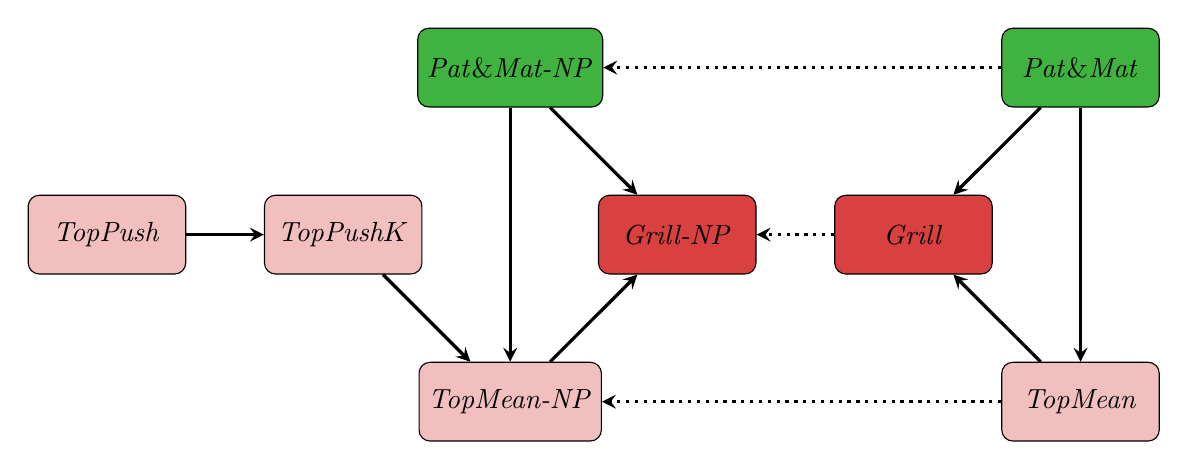
\begin{tikzpicture}[node distance=3cm]
    \node (node1) [bubble_red] {\toppush};
    \node (node2) [bubble_red, right of=node1] {\toppushk};
    \node (node3) [bubble_white, above right of=node2] {\patmatnp};
    \node (node4) [bubble_red, below right of=node2] {\topmeannp};
    \node (node5) [bubble_dark_red, below right of=node3] {\grillnp};
    \node (node6) [bubble_dark_red, right of=node5] {\grill};
    \node (node7) [bubble_white, above right of=node6] {\patmat};
    \node (node8) [bubble_red, below right of=node6] {\topmean};

    \draw [arrow_solid]  (node1) -- (node2);
    \draw [arrow_solid]  (node2) -- (node4);
    \draw [arrow_solid]  (node3) -- (node5);
    \draw [arrow_solid]  (node4) -- (node5);
    \draw [arrow_solid]  (node3) -- (node4);
    \draw [arrow_solid]  (node7) -- (node6);
    \draw [arrow_solid]  (node8) -- (node6);
    \draw [arrow_solid]  (node7) -- (node8);
    \draw [arrow_dotted] (node7) -- (node3);
    \draw [arrow_dotted] (node8) -- (node4);
    \draw [arrow_dotted] (node6) -- (node5);
  \end{tikzpicture}
  \caption{Summary of the methods from Section~\ref{sec:General framework}. Methods in green and light red are convex while methods in dark red are non-convex. Methods in light red are vulnerable to have the global minimum at~$\bm{w} = \bm{0}.$ Full (dotted) arrow pointing from one method to another show that the latter method has always (usually) smaller threshold.}
  \label{fig:thresholds}
\end{figure}


% ------------------------------------------------------------------------------
% Numerical Considerations
% ------------------------------------------------------------------------------
\section{Numerical considerations}


So far, we have performed a theoretical analysis of the presented methods. In this section, we present some numerical considerations as well.

\subsection{Gradient computation and variable reduction}


The decision variables in~\eqref{eq:General surrogate problem} are the normal vector of the separating hyperplane~$\bm{w}$ and the threshold~$t.$ To apply an efficient optimization method, we need to compute gradients. The simplest idea is to perform the gradient only with respect to~$\bm{w}$ and then recompute~$t.$ This was followed in~\cite{grill2016learning}. However, there is a more sophisticated way based on the implicit function theorem. For each~$\bm{w},$ the threshold~$t$ can be computed uniquely. We stress this dependence by writing~$t(\bm{w})$ instead of~$t.$ By doing so, we effectively remove the threshold~$t$ from the decision variables and~$\bm{w}$ remains the only decision variable. Note that the convexity is preserved. Then we can compute the derivative via the chain rule
\begin{equation}\label{eq:Derivatives}
  \begin{aligned}
    f(\bm{w})        & = \frac{1}{n^+}\sum_{i \in \I^+} l(t(\bm{w})  - \bm{w}^\top \bm{x}_i) + \frac{\lambda}{2}\norm{\bm{w}}^2, \\
    \nabla f(\bm{w}) & = \frac{1}{n^+}\sum_{i \in \I^+} l'(t(\bm{w}) - \bm{w}^\top \bm{x}_i)(\nabla t(\bm{w}) - \bm{x}_i) + \lambda \bm{w}.
  \end{aligned}
\end{equation}
The only remaining part is the computation of~$\nabla t(w).$ We show here an efficient computation for \toppushk and \patmat. For other methods, it can be performed in a similar manner. 

For \toppushk, we recall that the threshold~$t$ equals to the mean of~$K$ largest scores~$s = \bm{w}^\top \bm{x}_i,$ for all negative samples~$i \in \I^-.$ The locally, this is a linear function for which it is simple to compute derivatives
\begin{equation*}
  \nabla t =  \frac{1}{K} \sum_{j=1}^K \bm{x}_{l_j},
\end{equation*}
where~$l_1, l_2, \dots, l_K$ are indeces of~$K$ largest scores coresponding to the negative samples. To prevent unnecessary computations for~\eqref{eq:Derivatives}, we summarize the computations of derivatives for \toppushk in Algorithm~\ref{alg:Derivatives TopPushK}.

\begin{algorithm}[!ht]
  \begin{algorithmic}[1]
    \State Compute the scores~$s_i = \bm{w}^\top \bm{x}_i$ for all indices~$i \in \I.$
    \State Find~$K$ indices~$l_1,\dots,l_K$ where~$\bm{s}$ has the greatest values on~$\I^-.$
    \State Compute the threshold~$t = \frac{1}{k}\sum_{j=1}^K s_{l_j}.$
    \State Compute the threshold derivative~$\nabla t = \frac{1}{K}\sum_{j=1}^K \bm{x}_{l_j}.$
    \State Compute the derivative as~$\frac{1}{n_+}\sum_{i \in \I_+}l'\left( t- s_i\right) \left( \nabla t - \bm{x}_i\right)+\lambda\bm{w}.$
  \end{algorithmic}
  \caption{Efficient computation of~\eqref{eq:Derivatives} for \toppushk.}
  \label{alg:Derivatives TopPushK}
\end{algorithm}

For the \patmat method, the computation is slightly more difficult. The threshold~$t$ is defined through equation
\begin{equation*}
  \frac{1}{n}\sum_{i \in \I} l\left( \beta \left( \bm{w}^\top \bm{x}_i - t(\bm{w}) \right) \right) = \tau,
\end{equation*}
i.e. there is no explicit relation between the threshold~$t$ and the weights~$\bm{w}.$ However, differentiating this equation with respect to~$\bm{w}$ results in
\begin{equation*}
  \sum_{i \in \I} l'\left( \beta \left( \bm{w}^\top \bm{x}_i - t(\bm{w}) \right) \right)\left(\bm{x}_i - \nabla t(\bm{w}) \right) = 0,
\end{equation*}
and thus
\begin{equation*}
  \nabla t(\bm{w}) = \frac{\sum_{i \in \I} l'\left( \beta \left( \bm{w}^\top \bm{x}_i - t(\bm{w}) \right) \right)\bm{x}_i}{\sum_{i \in \I} l'\left( \beta \left( \bm{w}^\top \bm{x}_i - t(\bm{w}) \right) \right)}.
\end{equation*}
Similarly to the previous case, we present the efficient computation of~\eqref{eq:Derivatives} in Algorithm~\ref{alg:Derivatives PatMat}.

\begin{algorithm}[!ht]
  \begin{algorithmic}[1]
    \State Compute the scores~$s_i = \bm{w}^\top \bm{x}_i$ for all indices~$i \in \I.$
    \State Solve the equation~$\sum_{i \in \I}l(\beta(z_i-t))=n\tau$ for the threshold~$t.$
    \State Compute the threshold derivative~$\nabla t = \frac{\sum_{i\in \I}l'(\beta(s_i - t))\bm{x}_i}{\sum_{i \in \I}l'(\beta(s_i-t))}.$
    \State Compute the derivative as~$\frac{1}{n_+}\sum_{i \in \I_+}l'\left( t- s_i\right) \left( \nabla t - \bm{x}_i \right) + \lambda \bm{w}.$
  \end{algorithmic}
  \caption{Efficient computation of~\eqref{eq:Derivatives} for \patmat.}
  \label{alg:Derivatives PatMat}
\end{algorithm}


\subsection{Implementational details}

We recall that all methods fall into the framework of either~\eqref{eq:General problem} or~\eqref{eq:General surrogate problem}. Since the threshold~$t$ depends on the weights~$\bm{w},$ we can consider the decision variable to be only~$\bm{w}.$ Then to apply a method, we implemented the iterative procedure described in Algorithm~\ref{alg:General algorithm}.
\begin{algorithm}[!ht]
  \begin{algorithmic}[1]
    \State Initialization:~$j_{\max},$~$\bm{w}^0.$
    \State Set~$j \gets 0.$  
    \While{$j \leq j_{\max}$}
      \State Compute the threshold~$t^j = t(\bm{w}^j).$
      \State Compute the gradient of the objectiv fuction according to~\eqref{eq:Derivatives}. 
      \State Apply the ADAM scheme~\cite{kingma2014adam} to get the descent step~$\bm{p}^j.$
      \State Update the weights~$\bm{w}^{j+1} \gets \bm{w}^j - \bm{p}^j.$
      \State Update~$j \gets j + 1.$
    \EndWhile
    \State Compute the threshold~$t^{j_{\max}} = t(\bm{w}^{j_{\max}}).$
    \State Return~$\bm{w}^{j_{\max}},$~$t^{j_{\max}}.$
  \end{algorithmic}
  \caption{General gradient descent based procedure.}
  \label{alg:General algorithm}
\end{algorithm}


% ------------------------------------------------------------------------------
% Numerical experiments
% ------------------------------------------------------------------------------
\section{Numerical experiments}

\subsection{Dataset description}

For the numerical results, we considered nine datasets summarized in Table~\ref{tab:counts}. Five of them are standard and can be downloaded from the UCI repository. Datasets Ionosphere~\cite{sigillito1989ionosphere} and Spambase are small, Hepmass~\cite{baldi2016hepmass} contains a large number of samples while Gisette~\cite{guyon2005gisette} contains a large number of features. To make the dataset more difficult, we created Hepmass 10\% dataset which is a random subset of the Hepmass dataset and reduces the fraction of positive samples from 50\% to 10\%.

Besides these datasets, we also considered two real-world datasets CTA and NetFlow obtained from existing network intrusion detection systems. The first one, further called CTA, was created by the Cisco's Cognitive Threat Analytics engine~\cite{cisco2014cta} which analyzes HTTP proxy logs (typically produced by proxy servers located on a network perimeter). The second one, further called NetFlow, was collected by the NetFlow anomaly detection engine~\cite{rehak2009adaptive,garcia2014empirical} which processes NetFlow~\cite{cisco2004netflow} records exported by routers and other network traffic shaping devices. All samples were manually labelled by experienced Cisco analysts. Therefore it is safe to assume that samples labelled as malicious are indeed malicious. However, it may happen that some samples labelled as legitimate can be actually malicious, which typically happens due to the new type of attack (malware) with a different behaviour from what has been seen in the past. To study classifier robustness to this type of errors, we follow the experimental protocol of~\cite{grill2016learning} and besides the original dataset, we inject artificial noise \emph{MLT} which corresponds to the situation where security analysts have failed to identify 50\% of attack types and partially mislabelled the other 50\% attack types. Thus, some positive samples are either missing or have a wrong (negative) label in the training and validation set. However, they are present in the testing set. A more precise description of the used datasets and the data generating and labelling process is in~\cite{grill2016learning}.

\begin{table}[t]
  \caption{Structure of the used datasets. The training, validation and testing sets show the number of features~$m,$ minibatches~$n_{\min},$ samples~$n$ and the fraction of positive samples~$\frac{n^+}{n}.$}
  \label{tab:counts}
  \centering
  \resizebox{\textwidth}{!}{
    \begin{tabular}{@{} lllllllll @{}}
      \toprule
                  &       &            & \multicolumn{2}{c}{\bf Training} & \multicolumn{2}{c}{\bf Validation} & \multicolumn{2}{c}{\bf Testing} \\
      \cmidrule(lr){4-5} \cmidrule(lr){6-7} \cmidrule(l){8-9}
                  &~$m$   &~$n_{\min}$ &~$n$                              &~$\frac{n^+}{n}$                    &~$n$                                &~$\frac{n^+}{n}$ &~$n$       &~$\frac{n^+}{n}$ \\
      \midrule
      Ionosphere  & 34    & 1          & 175                              & 36.0\%                             & 88                                 & 35.2\%          & 88        & 36.4\% \\
      Spambase    & 57    & 1          & 2~300                            & 39.4\%                             & 1~150                              & 39.4\%          & 1~151     & 39.4\% \\
      Gisette     & 5~001 & 1          & 6~000                            & 50.0\%                             & 500                                & 50.0\%          & 500       & 50.0\% \\
      Hepmass     & 28    & 40         & 5~250~000                        & 50.0\%                             & 2~625~040                          & 50.0\%          & 2~624~960 & 50.0\% \\
      Hepmass 10  & 28    & 40         & 2~916~636                        & 10.0\%                             & 1~458~320                          & 10.0\%          & 1~458~240 & 10.0\% \\
      CTA         & 34    & 26         & 263~796                          & 2.1\%                              & 263~796                            & 2.2\%           & 527~488   & 2.1\% \\
      CTA MLT     & 34    & 9          & 91~314                           & 0.3\%                              & 91~314                             & 0.3\%           & 182~592   & 2.1\% \\
      NetFlow     & 25    & 8          & 142~676                          & 8.7\%                              & 142~674                            & 8.7\%           & 285~454   & 8.6\% \\
      NetFlow MLT & 25    & 8          & 145~260                          & 2.7\%                              & 145~261                            & 2.8\%           & 285~508   & 8.6\% \\
      \bottomrule
    \end{tabular}
  }
\end{table}


\subsection{Performance criteria}

In Section~\ref{sec:General framework}, we described three classes of methods, each optimizing a different criterion. Utilizing the ``Criterion'' column in Table~\ref{tab:Methods}, we summarize these three criteria in Table~\ref{tab:criteria}. We recall that the precision and recall are for a threshold~$t$ defined by
\begin{equation*}
  \begin{aligned}
    \precision & = \frac{\tp(\bm{w},t)}{\tp(\bm{w},t)+\fp(\bm{w},t)}, &
    \recall    & = \frac{\tp(\bm{w},t)}{\tp(\bm{w},t)+\fn(\bm{w},t)}.
  \end{aligned}
\end{equation*}
We will show the Precision-Recall (PR) and the Precision-$\tau$ (P$\tau$) curves. The former is a well-accepted visualization for highly unbalanced data~\cite{davis2006relationship} while the latter better reflects that the methods concentrate only on the top of the scores.

\begin{table}[!ht]
  \caption{The criteria for the three classes from Section~\ref{sec:General framework}.}
  \label{tab:criteria}
  \centering
  \begin{tabular}{@{} ll @{}}
    \toprule
    \bf Name           & \bf Description \\
    \midrule
    Positives@Top      & Fraction of positives above the largest negative~\eqref{eq:TopPush maximization}. \\
    Positives@Quantile & Fraction of positives above the~$\tau$-quantile~\eqref{eq:AATP original}. \\
    Positives@NP       & Fraction of positives above the Neyman-Pearson threshold~\eqref{eq:Neyman-Pearson}. \\
    \bottomrule
  \end{tabular}
\end{table}


\subsection{Hyperparameter choice}

In Algorithm~\ref{alg:General algorithm}, we described the iterative procedure used for all of the methods from Section~\ref{sec:General framework}. Only for \grill and \grillnp method we stick to the original paper~\cite{grill2016learning} and apply the projection of weights~$\bm{w}$ onto the~$l_2$-unit ball after each gradient step (this is not advised for other methods as convexity would be lost). All methods used the hinge surrogate~\eqref{eq:Surrogates} and the maximal number of iterations were set to~$1000$ iterations. Moreover, for large datasets, we replaced the standard gradient descent by its stochastic counterpart~\cite{bottou2010large} where the threshold~$t^j$ and the gradient are computed only on a part of the dataset called a minibatch.

In the experimental part, we use the following sets of hyperparameters for the methods
\begin{equation*}
  \begin{aligned}
    \tau    & \in \{0.01,\ 0.02,\ 0.03,\ 0.04,\ 0.05,\ 0.1 \}, &
    \beta   & \in \{0.0001,\ 0.001,\ 0.01,\ 0.1,\ 1,\ 10 \}, \\
    \lambda & \in \{0,\ 0.00001,\ 0.0001,\ 0.001,\ 0.01,\ 0.1 \}, &
    K       & \in \{1,\ 3,\ 5,\ 10,\ 15,\ 20 \}.
  \end{aligned}
\end{equation*}
Since \toppushk, \patmat and \patmatnp use two hyperparameters, we fixed~$\lambda=0.001$ for these methods to have only six hyperparameters for all methods. For all datasets, we choose the  hyperparameter which minimized the corresponding criterion from Table~\ref{tab:Methods} on the validation set. The results are computed on the testing set which was not used during training the methods.

Note that \toppush was originally implemented in the dual. However, to allow for the same framework and for the stochastic gradient descent, we implemented it in the primal. These two approaches are, at least theoretically, equivalent. 


\subsection{Results}

In this section, we present the numerical results. Note that all results are computed on the testing set which was not available during training. We run the algorithms from~$\bm{w}^0=\bm{0}$ and from a randomly generated point in the interval~$[-1,1].$ Since the former showed a better performance in~$58.7\%$ cases, we show only the results starting from zero.

Having shown a good performance of the methods, we focus on their comparison. Since all methods optimize one of the criteria from Table~\ref{tab:criteria}, we base the comparison on these criteria. First, we consider 14 methods (we count different values of~$\tau$ as a different method) as depicted in Table~\ref{tab:results2}. Note that \toppushk for~$K=1$ reduces to the classical \toppush. For each dataset and each method, we evaluated criteria from Table~\ref{tab:criteria}. For each dataset and criterion, we computed the rank of all methods and averaged them with respect to all datasets. Rank 1 refers to the best performance for given criteria while rank 14 is the worst. Since criteria are in columns, the comparison among methods is column-wise. The best method is depicted in dark green and comparable methods (at most one rank away) are depicted in light green.

\begin{table}[t]
  \caption{The average rank of all methods across all datasets on the criteria from Table~\ref{tab:criteria}. Rank~1 is the best and rank~14 is the worst. This evaluation is performed for each criterion. Dark green depicts the best method while light green depicts comparable methods.}
  \label{tab:results2}
  \centering
  \resizebox{\textwidth}{!}{
    \begin{tabular}{@{} lllllll @{}}
      \toprule
                 &             & \bf Positives@Top           & \multicolumn{2}{c}{\bf Positives@Quantile} & \multicolumn{2}{c}{\bf Positives@NP} \\
      \cmidrule(r){4-5} \cmidrule(l){6-7}
                 &             &                             &~$\tau=0.01$                                &~$\tau=0.03$                             &~$\tau=0.01$                 &~$\tau=0.03$ \\
      \midrule
      \toppush   &             &~$5.5$                       &~$8.1$                                      &~$8.4$                                   &~$8.3$                       &~$9.3$ \\
      \toppushk  &             & \cellcolor{mygreen!75}$4.2$ &~$7.2$                                      &~$8.4$                                   &~$7.4$                       &~$7.3$ \\
      \grill     &~$\tau=0.01$ &~$10.1$                      &~$9.7$                                      &~$11.2$                                  &~$11.4$                      &~$10.9$ \\
                 &~$\tau=0.03$ &~$8.9$                       &~$10.1$                                     &~$10.3$                                  &~$11.1$                      &~$10.1$ \\
      \patmat    &~$\tau=0.01$ &~$8.1$                       &~$7.1$                                      &~$6.8$                                   &~$5.6$                       &~$6.1$ \\
                 &~$\tau=0.03$ &~$6.3$                       &~$6.8$                                      &~$5.5$                                   &~$5.9$                       &~$5.2$ \\
      \topmean   &~$\tau=0.01$ &~$9.1$                       &~$10.3$                                     &~$8.8$                                   &~$9.9$                       &~$10.7$ \\
                 &~$\tau=0.03$ &~$9.4$                       &~$9.1$                                      &~$8.3$                                   &~$9.8$                       &~$10.2$ \\
      \grillnp   &~$\tau=0.01$ &~$9.6$                       &~$8.4$                                      &~$9.4$                                   &~$10.2$                      &~$9.8$ \\
                 &~$\tau=0.03$ &~$10.8$                      &~$8.5$                                      &~$9.3$                                   &~$9.3$                       &~$7.6$ \\
      \patmatnp  &~$\tau=0.01$ &~$6.6$                       & \cellcolor{mygreen!30}$5.0$                & \cellcolor{mygreen!75}$3.4$             & \cellcolor{mygreen!75}$2.8$ &~$4.4$ \\
                 &~$\tau=0.03$ &~$6.9$                       &~$5.4$                                      &~$4.7$                                   &~$4.3$                       & \cellcolor{mygreen!75}$3.2$ \\
      \topmeannp &~$\tau=0.01$ & \cellcolor{mygreen!30}$4.9$ &~$5.3$                                      &~$6.3$                                   &~$5.9$                       &~$6.0$ \\
                 &~$\tau=0.03$ & \cellcolor{mygreen!30}$4.6$ & \cellcolor{mygreen!75}$4.1$                & \cellcolor{mygreen!30}$4.0$             & \cellcolor{mygreen!30}$2.9$ & \cellcolor{mygreen!30}$4.1$ \\
      \bottomrule
    \end{tabular}
  }
\end{table}

\noindent Based on the results in the Table~\ref{tab:results2}, we make several observations:
\begin{itemize}
  \item \toppushk performs better than \toppush. We relate this to the greater stability given by considering~$K$ largest negatives in \toppushk instead of~$1$ in \toppush. This may have alleviated the problems with~$\bm{w}=\bm{0}$ as suggested in Theorem~\ref{thm:large_t}.
  \item Neither \grill nor \grillnp perform well. We believe that this is due to the lack of convexity as indicated in Theorem~\ref{thm:convex} and the discussion thereafter.
  \item \topmean does not perform well either. Since the thresholds~$\tau$ are small, then~$\bm{w}=\bm{0}$ is the global minimum as proved in Corollary~\ref{cor:topmean}.
  \item \toppush and \toppushk methods work better on the Positives@Top criterion. This complies with the theory as these methods were designed for this criterion.
  \item \patmat, \patmatnp and \topmeannp methods work better on the Positives@Quantile and Positives@NP criterion. This complies with the theory as these methods were designed for one of these criteria.
\end{itemize}

\noindent In Table~\ref{tab:fails} we investigate the impact of~$\bm{w}=\bm{0}$ as a potential global minimum. Each method was optimized for six different values of hyperparameters. The table depicts the condition under which the final value has a lower objective that~$\bm{w}=\bm{0}.$ Thus, \cmark\ means that it is always better while \xmark\ means that the algorithm made no progress from the starting point~$\bm{w} =0.$ The latter case implies that~$\bm{w}=\bm{0}$ seems to be the global minimum. We make the following observations:
\begin{itemize}
  \item \toppushk has a lower number of successes than \patmatnp which corresponds to Figure~\ref{fig:thresholds} showing that the latter method has a lower threshold.
  \item Similarly, Figure~\ref{fig:thresholds} states that the methods from Section~\ref{subsec:Accuracy at the top} has a higher threshold than their Neyman-Pearson variants from Section~\ref{subsec:Hypothesis testing}. This is documented in the table as the latter have a higher number of successes.
  \item \patmat and \patmatnp are the only methods which succeeded at every dataset for some hyperparameter. Moreover, for each dataset, there was some~$\beta_0$ such that these methods were successful if and only if~$\beta\in(0,\beta_0).$ This is in agreement with Theorem~\ref{thm:patmat_zero}. The only exception was Spambase which we attribute to numerical errors.
  \item \topmean fails everywhere which agrees with Corollary~\ref{cor:topmean}. The only exception is the case of~$\tau=3\%$ and CTA which has only~$2.1\%$ positive samples. This again agrees with Corollary~\ref{cor:topmean}.
\end{itemize}

\begin{table}[t]
  \caption{Necessary hyperparameter choice for the solution to have a better objective than zero. \cmark\ means that the solution was better than zero for all hyperparameters while \xmark\ means that it was worse for all hyperparameters.}
  \label{tab:fails}
  \centering
  \resizebox{\textwidth}{!}{
    \begin{tabular}{@{} llcccccc @{}}
      \toprule
                 &             & \bf Ionosphere & \bf Spambase    & \bf Gisette     & \bf Hepmass   & \bf CTA       & \bf NetFlow \\
      \midrule
      \toppush   &             & \cmark         & \xmark          & \cmark          & \xmark        & \cmark        & \xmark \\
      \toppushk  &             & \cmark         & \xmark          & \cmark          & \xmark        & \cmark        & \xmark \\
      \grill     &~$\tau=0.01$ & \xmark         & \xmark          & \xmark          & \xmark        & \cmark        & \cmark \\
                 &~$\tau=0.03$ & \cmark         & \xmark          & \xmark          & \xmark        & \cmark        & \cmark \\
      \patmat    &~$\tau=0.01$ &~$\beta\le0.1$  &~$\beta=0.001$   &~$\beta\le0.001$ &~$\beta\le0.1$ &~$\beta\le0.1$ &~$\beta\le0.1$ \\
                 &~$\tau=0.03$ &~$\beta\le0.1$  &~$\beta=0.01$    &~$\beta\le0.001$ &~$\beta\le0.1$ &~$\beta\le0.1$ &~$\beta\le0.1$ \\
      \topmean   &~$\tau=0.01$ & \xmark         & \xmark          & \xmark          & \xmark        & \xmark        & \xmark \\
                 &~$\tau=0.03$ & \xmark         & \xmark          & \xmark          & \xmark        & \cmark        & \xmark \\
      \grillnp   &~$\tau=0.01$ & \cmark         & \xmark          & \xmark          & \xmark        & \cmark        & \cmark \\
                 &~$\tau=0.03$ & \cmark         & \xmark          & \xmark          & \xmark        & \cmark        & \cmark \\
      \patmatnp  &~$\tau=0.01$ &~$\beta\le1$    &~$\beta=0.01$    & \cmark          &~$\beta\le0.1$ & \cmark        &~$\beta\le0.1$ \\
                 &~$\tau=0.03$ &~$\beta\le1$    &~$\beta=0.1$     & \cmark          &~$\beta\le0.1$ & \cmark        &~$\beta\le0.1$ \\
      \topmeannp &~$\tau=0.01$ & \cmark         &~$\lambda=0.001$ & \cmark          & \xmark        & \cmark        & \xmark \\
                 &~$\tau=0.03$ & \cmark         & \cmark          & \cmark          & \xmark        & \cmark        & \xmark \\
      \bottomrule
    \end{tabular}
  }
\end{table}

\noindent In Figure~\ref{fig:ptau} we present the P$\tau$ curves which show the precision at the top~$\tau$-quantile. They are equivalent to the well-known PR curves. Each row corresponds to one dataset (NetFlow top row, Gisette middle row and Hepmass bottom row), the left column shows the whole interval for the quantile~$\tau\in[0,1]$ while the right one is its zoomed version to~$\tau\in[0,0.01].$ We show the \toppushk, \patmat, \patmatnp and \topmeannp methods which perform the best as can be seen from the previous results. Note that the right column is more important as all these method focus on maximizing the accuracy only on the top of the dataset, which precisely corresponds to small values of~$\tau.$ The \patmat and \patmatnp methods perform the best on larger quantiles. \toppushk performs reasonably well for large quantiles while its performance increases with decreasing~$\tau.$ In most cases, the precision is~$1$ when~$\tau$ is sufficiently small.
\begin{figure}[p]
  \begin{tikzpicture}
    \pgfplotsset{}
    \begin{groupplot}[group style = {group size = 2 by 3, horizontal sep = 5pt, vertical sep = 5pt},
                            ymin = 0, ymax = 1.05, ytick = {0,0.2,0.4,0.6,0.8,1}, grid  = major,
                            grid style={dashed, gray!50, very thin}]
      \nextgroupplot[col1, xticklabels={}, ylabel={Precision}, legend style = legendStyle]
          \addplot [line1] table[x index=0, y index=1] {\DataNetflow}; \addlegendentry{\toppushk}
          \addplot [line2] table[x index=0, y index=2] {\DataNetflow}; \addlegendentry{\patmat}
          \addplot [line3] table[x index=0, y index=3] {\DataNetflow}; \addlegendentry{\patmatnp}
          \addplot [line4] table[x index=0, y index=4] {\DataNetflow}; \addlegendentry{\topmeannp}
      \nextgroupplot[col3, xticklabels={}, yticklabels={}]
          \addplot [line1] table[x index=0, y index=1] {\DataNetflowSmall};
          \addplot [line2] table[x index=0, y index=2] {\DataNetflowSmall};
          \addplot [line3] table[x index=0, y index=3] {\DataNetflowSmall}; 
          \addplot [line4] table[x index=0, y index=4] {\DataNetflowSmall};            
      \nextgroupplot[col1, xticklabels={}, ylabel={Precision}] 
          \addplot [line1] table[x index=0, y index=1] {\DataGisette}; 
          \addplot [line2] table[x index=0, y index=2] {\DataGisette}; 
          \addplot [line3] table[x index=0, y index=3] {\DataGisette}; 
          \addplot [line4] table[x index=0, y index=4] {\DataGisette};   
      \nextgroupplot[col3, xticklabels={}, yticklabels={}] 
          \addplot [line1] table[x index=0, y index=1] {\DataGisetteSmall}; 
          \addplot [line2] table[x index=0, y index=2] {\DataGisetteSmall}; 
          \addplot [line3] table[x index=0, y index=3] {\DataGisetteSmall}; 
          \addplot [line4] table[x index=0, y index=4] {\DataGisetteSmall};   
      \nextgroupplot[col1, xlabel={$\tau$}, ylabel={Precision}]
          \addplot [line1] table[x index=0, y index=1] {\DataHepmass};
          \addplot [line2] table[x index=0, y index=2] {\DataHepmass};
          \addplot [line3] table[x index=0, y index=3] {\DataHepmass}; 
          \addplot [line4] table[x index=0, y index=4] {\DataHepmass};   
      \nextgroupplot[col3, xlabel={$\tau$}, yticklabels={}]
          \addplot [line1] table[x index=0, y index=1] {\DataHepmassSmall};
          \addplot [line2] table[x index=0, y index=2] {\DataHepmassSmall};
          \addplot [line3] table[x index=0, y index=3] {\DataHepmassSmall}; 
          \addplot [line4] table[x index=0, y index=4] {\DataHepmassSmall};   
    \end{groupplot}
    \node at ($(group c2r1) + (-3.5,3.3)$) {\ref{grouplegendA}}; 
  \end{tikzpicture}
  \caption{P$\tau$ curves for datasets NetFlow (top row), Gisette (middle row) and Hepmass (bottom row) and two different zooms of~$\tau\in[0,1]$ and~$\tau\in[0,0.01]$ (columns).}
  \label{fig:ptau}
\end{figure}

The final Table~\ref{tab:time} depicts the time needed for one iteration in milliseconds. We show four selected representative methods. Note that the time is relatively stable and even for most of the datasets it is below one millisecond. Thus, the whole optimization for one hyperparameter (without loading and evaluation) can be usually performed within one second.
\begin{table}[!ht]
  \caption{Time in miliseconds needed for one iteration.}
  \label{tab:time}
  \centering
  \begin{tabular}{@{} lllllll @{}}
    \toprule
              & \bf Ionosphere & \bf Spambase & \bf Gisette & \bf Hepmass & \bf CTA & \bf NetFlow \\
    \midrule
    \toppushk &~$0.0$          &~$0.1$        &~$22.3$      &~$5.6$       &~$0.5$   &~$0.9$ \\
    \grill    &~$0.0$          &~$0.1$        &~$41.5$      &~$6.2$       &~$0.5$   &~$1.1$ \\
    \patmat   &~$0.0$          &~$0.2$        &~$38.4$      &~$8.4$       &~$0.4$   &~$1.1$ \\
    \topmean  &~$0.0$          &~$0.2$        &~$43.9$      &~$7.1$       &~$0.4$   &~$0.9$ \\
    \bottomrule
  \end{tabular}
\end{table}



% ------------------------------------------------------------------------------
% Conclusion
% ------------------------------------------------------------------------------
\section{Conclusion and future work}


In this work we achieved the following results:
\begin{itemize}
  \item We presented a unified framework for the three criteria from Section~\ref{sec:General framework}.
  \item We showed which known methods (\toppush, \grill) fall into our framework and derived both completely new methods (\patmat, \patmatnp, \topmean) and modifications of known methods (\toppushk, \grillnp, \topmeannp).
  \item We performed a theoretical analysis of the methods. We showed that both known methods suffer from certain disadvantages. While \toppush is sensitive to outliers, \grill is non-convex.
  \item We performed a numerical comparison where we showed a good and fast performance. The methods converge within seconds on datasets with 5 million training samples.
  \item The extensive theoretical analysis is supported by the numerical analysis.
\end{itemize}
Based on the results, we recommend using \toppushk or \topmeannp for extremely small~$\tau.$ For larger~$\tau,$ we recommend using \patmat or \patmatnp as they are convex and do not suffer from problems at~$\bm{w}=\bm{0}.$

\subsection{Future work}

All presented methods cover only the case where the linear classification is sufficient. However, many problems are not linearly separable and then the non-linear classifiers are needed. One could say that the easiest way how to incorporate non-linearity in the formulation of our framework~\eqref{eq:General problem} is to replace the linear classifier by the non-linear one. The problem is that it would only lead to the loss of the convexity and the task will be hardly solvable. Nevertheless, we can use existing theory to get some inspiration for our future work. The key point is to realize that our framework is really similar to the primal formulation of the famous support vector machines~\cite{cortes1995support}. The classical way how to incorporate non-linearity into SVM is to derive the dual formulation~\cite{boyd2004convex} corresponding to the primal problem and use the kernels methods~\cite{scholkopf2001learning}. The main problem of this approach is that dimension of the dual formulation depends on the number of samples and as a consequence, it is hard to solve SVM in dual for large datasets. However, there are two main ways how to increase the scalability which are used for SVM.

\begin{itemize}
  \item The first way is to reduce the number of data samples. This approach uses the well-known feature of SVM that the resulting classifier is determined only by the subset of all training samples called support vectors. Since the classifier is characterized only by support vectors and the rest of the samples has no effect on the classification result, it is possible to reduce the training data set to a set of support vectors. Data reduction can easily be used in the testing phase since a set of support vectors is known at this stage. On the other hand, it is hard to use this property in the training phase because it is generally difficult to determine which samples are support vectors during this phase. However, there are for example screening methods~\cite{ogawa2013safe,wang2014scaling} which solve this problem and try to identify non-support vectors to reduce the number of samples during the training phase.

  \item The second way is to improve the training method. Such an improvement can be made, for example, by the coordinate descent method~\cite{chang2008coordinate,hsieh2008dual}. The key idea of this approach is to update only one variable (or a few) instead of updating all variables at once. Solving the subproblem for just one variable is much easier than solving the whole dual task. In addition, the subproblem of one variable sometimes has an analytical solution and can be solved at a constant time.
\end{itemize}

\noindent Our main object of interest for the future is to properly derive and solve dual formulations of all methods described in this work.

% ------------------------------------------------------------------------------
% Appendix
% ------------------------------------------------------------------------------
\appendix
\section{Additional results and proofs}\label{app:Additional results and proofs}

Here, we provide additional results and proofs of results mentioned in the main body. For convenience, we repeat the result statements.

\subsection{Equivalence of~\eqref{eq:AATP original},~\eqref{eq:AATP robust} and~\eqref{eq:AATP}}

To show this equivalence, we will start with an auxiliary lemma.

\begin{lemma}\label{lemma:fnfp_equivalence}
  Denote by~$t$ the exact quantile from~\eqref{eq:Empirical quantile}. Then for all~$\alpha\in[0,1]$ we have
  \begin{equation*}
    \fp(\bm{w},t) = \alpha \fp(\bm{w},t) + (1-\alpha)\fn(\bm{w},t) + (1-\alpha)(n\tau - n^+) + (1-\alpha)(q - 1),
  \end{equation*}
  where~$q:= \#\{\bm{x} \in \X \mid \bm{w}^\top \bm{x} = t\}.$
\end{lemma}

\begin{proof}
  By the definition of the quantile we have
  \begin{equation*}
    \tp(\bm{w},t) + \fp(\bm{w},t) = n \tau + q - 1.
  \end{equation*}
  This implies
  \begin{equation*}
    \fp(\bm{w},t) = n \tau + q - 1 -\tp(\bm{w},t)
                  = n \tau + q - 1 - n^{+} +\fn(\bm{w},t).
  \end{equation*}
  From this relation we deduce
  \begin{align*}
    \fp(\bm{w},t) & = \alpha \fp(\bm{w},t) + (1-\alpha)\fp(\bm{w},t)
                    = \alpha \fp(\bm{w},t) + (1-\alpha)\left(\fn(\bm{w},t) + n\tau - n^+ + q - 1\right)\\
                  & = \alpha \fp(\bm{w},t) + (1-\alpha)\fn(\bm{w},t) + (1-\alpha)\left(n\tau - n^+\right) + (1-\alpha)\left(q - 1\right),
  \end{align*}
  which is precisely the lemma statement.
\end{proof}

\subsection{Results related to convexity and continuity}


\TheoremRef{thm:convex}{
  If the threshold~$t$ is a convex function of the weights~$\bm{w},$ then function~$f(\bm{w}) = \fns(\bm{w}, t(\bm{w}))$ is convex.
}
\begin{proof}
  Due to the definition of the surrogate counts~\eqref{eq:Counts surrogates}, the objective of~\eqref{eq:General surrogate problem} equals to
  \begin{equation*}
   \frac{1}{n^+}\sum_{i \in \I^+} l\left(t(\bm{w})-\bm{w}^\top \bm{x}_i\right).
  \end{equation*}
  Here we write~$t(\bm{w})$ to stress the dependence of~$t$ on~$\bm{w}.$ Since~$\bm{w} \mapsto t(\bm{w})$ is a convex function, we also have that~$\bm{w} \mapsto t(\bm{w})-\bm{w}^\top \bm{x}$ is a convex function. From its definition, the surrogate function~$l$ is convex and non-decreasing. Since a composition of a convex function with a non-decreasing convex function is a convex function, this finishes the proof.
\end{proof}

\begin{lemma}\label{lemma:Convexity of surrogate quantiles}
  Functions~$\bm{w} \mapsto \bar t_{\rm Q}(\bm{w})$ defined in~\eqref{eq:Surrogate quantile} and~$\bm{w} \mapsto \bar t_{\rm NP}(\bm{w})$ defined in~\eqref{eq:Surrogate quantile Neyman-Pearson} are convex.
\end{lemma}

\begin{proof}
  We will show this result only for the function~$\bm{w} \mapsto \bar t_{\rm Q}(\bm{w}).$ For the second function, it can be shown in a identical way. This former function is defined via the implicit equation
  \begin{equation*}
    g(\bm{w}, t) := \frac{1}{n} \sum_{i \in\I} l\left(\bm{w}^\top \bm{x}_i - t \right) - \tau = 0.
  \end{equation*}
  Since~$l$ is convex, we immediately obtain that~$g$ is jointly convex in both variables.

  To show the convexity, consider~$\bm{w}_1,$~$\bm{w}_2$ and the corresponding~$t_1 = \bar t_{\rm Q}(\bm{w}_1),$~$t_2 = \bar t_{\rm Q}(\bm{w}_2).$ Note that this implies
  \begin{equation}\label{eq:convexity_proof}
    g(\bm{w}_1, t_1) = g(\bm{w}_2,t_2)=0. 
  \end{equation}
  Then for any~$\lambda \in [0,1]$ we have
  \begin{equation}\label{eq:proof_conv1}
    g(\lambda \bm{w}_{1} + (1 - \lambda)\bm{w}_{2}, \;\lambda t_{1} + (1 - \lambda)t_{2}) \leq \lambda g(\bm{w}_{1}, t_{1}) + (1 - \lambda)g(\bm{w}_{2},t_{2}) = 0,
  \end{equation}
  where the inequality follows from the convexity of~$g$ and the equality~\eqref{eq:convexity_proof}. From the definition of the surrogate quantile we have
  \begin{equation}\label{eq:proof_conv2}
    g(\lambda\bm{w}_{1}+(1-\lambda)\bm{w}_{2},\bar{t}_{\rm Q}(\lambda\bm{w}_{1}+(1-\lambda)\bm{w}_{2}))=0.
  \end{equation}
  Since~$g$ is non-increasing in the second variable, from~\eqref{eq:proof_conv1} and~\eqref{eq:proof_conv2} we deduce
  \begin{equation*}
  \bar{t}_{\rm Q}(\lambda\bm{w}_{1}+(1-\lambda)\bm{w}_{2})\le\lambda t_{1}+(1-\lambda)t_{2} =\lambda\bar{t}_{\rm Q}(\bm{w}_{1})+(1-\lambda)\bar{t}_{\rm Q}(\bm{w}_{2}),
  \end{equation*}
  which implies that function~$\bm{w} \mapsto \bar t_{\rm Q}(\bm{w})$ is convex.
\end{proof}

\begin{lemma}\label{lemma:quantile_continuous}
  Functions~$\bm{w}\mapsto t_{\rm Q}(\bm{w})$ defined in~\eqref{eq:Empirical quantile} and~$\bm{w}\mapsto t_{\rm NP}(\bm{w})$ defined in~\eqref{eq:Empirical quantile Neyman-Pearson} are Lipschitz continuous.
\end{lemma}

\begin{proof}
  The quantile~$t_{\rm Q}(\bm{w})$ equals to one or more scores~$z=\bm{w}^\top \bm{x}.$ This implies that function~$\bm{w}\mapsto t_{\rm Q}(\bm{w})$ is piecewise linear which implies that it is Lipschitz continuous.
\end{proof}


\subsection{Results related to the global minima at zero}

\TheoremRef{thm:large_t}{
  Consider any of these methods: \toppush, \toppushk, \topmean or \topmeannp. Fix any~$\bm{w}$ and denote the corresponding threshold~$t.$ If we have
  \begin{equation}\label{eq:w_zero_nn}
    t \ge \frac{1}{n^+} \sum_{i^+ \in \I^+} \bm{w}^\top \bm{x}_i,
  \end{equation}
  then~$f(\bm{0}) \le f(\bm{w}).$
}

\begin{proof}
  First note that due to~$l(0) = 1$ and the convexity of~$l$ we have~$l(s) \ge 1 + cs,$ where~$c$ equals to the derivative of~$l$ at~$0.$ Then we have
  \begin{align}
    f(\bm{w}) & \ge \frac{1}{n^+} \fns(\bm{w}, t)
                =   \frac{1}{n^+} \sum_{i \in \I^+}l(t - \bm{w}^\top \bm{x}_i)
                \ge \frac{1}{n^+} \sum_{i \in \I^+}(1 + c(t - \bm{w}^\top \bm{x}_i)) \\
              & = 1 + \frac{c}{n^+}\sum_{i \in \I^+}(t - \bm{w}^\top \bm{x}_i)
                = 1 + ct - \frac{c}{n^+}\sum_{i \in \I^+}\bm{w}^\top \bm{x}_i
                \ge 1,
  \end{align}
  where the last inequality follows from~\eqref{eq:w_zero_nn}. Now we realize that for any method from the statement, the corresponding threshold for~$\bm{w}=0$ equals to~$t=0,$ and thus~$f(\bm{0})=1.$ But then~$f(\bm{0})\le f(\bm{w}),$ which finishes the proof.
\end{proof}


\TheoremRef{thm:patmat_zero}{
  Consider the \patmat or \patmatnp method with the hinge surrogate and no regularization. Assume that for some~$\bm{w}$ we have
  \begin{equation}\label{eq:patmat_zero_nn}
    \frac{1}{n^+} \sum_{i \in \I^+} \bm{w}^\top \bm{x}_i > \frac{1}{n^-}\sum_{j \in \I^-}\bm{w}^\top \bm{x}_j.
  \end{equation}
  Then there exists some~$\beta>0$ such that~$f(\bm{w})<f(\bm{0}).$
}

\begin{proof}
  Define
  \begin{align*}
    s_{\min} & = \min_{i \in \I} \bm{w}^\top \bm{x}_i,  &
    \bar{s}  & = \frac{1}{n} \sum_{i \in \I} \bm{w}^\top \bm{x}_i, &
    s_{\max} & = \max_{i \in \I} \bm{w}^\top \bm{x}.
  \end{align*}
  Then we have the following chain of relations
  \begin{equation}\label{eq:patmat_zero_aux0}
    \begin{aligned}
    \bar{s} & = \frac{1}{n} \sum_{i \in \I} \bm{w}^\top \bm{x}_i
              = \frac{1}{n} \sum_{i \in \I^+} \bm{w}^\top \bm{x}_i + \frac{1}{n} \sum_{i \in \I^-} \bm{w}^\top \bm{x}_i
              < \frac{1}{n} \sum_{i \in \I^+} \bm{w}^\top \bm{x}_i + \frac{n^-}{nn^+} \sum_{i \in \I^+} \bm{w}^\top \bm{x}_i \\
            & = \frac{1}{n} \left(1 + \frac{n^-}{n^+}\right) \sum_{i \in \I^+} \bm{w}^\top \bm{x}_i
              = \frac{1}{n} \frac{n^+ + n^-}{n^+} \sum_{i \in \I^+} \bm{w}^\top \bm{x}_i
              = \frac{1}{n^+} \sum_{i \in \I^+} \bm{w}^\top \bm{x}_i.
    \end{aligned}
  \end{equation}
  The only inequality follows from~\eqref{eq:patmat_zero_nn} and the last equality follows from~$n^+ + n^- = n.$

  Due to~\eqref{eq:patmat_zero_nn} we observe~$s_{\min}<\bar{s}<s_{\max}.$ Then we can define
  \begin{align*}
    \beta & = \min \left\{\frac{\tau}{\bar{s} - s_{\min}}, \frac{1 - \tau}{s_{\max}-\bar{s}} \right\}, &
    t     & = \frac{1-\tau}{\beta} + \bar{s}.
  \end{align*}
  We note that~$\beta>0.$ At the same time we obtain
  \begin{equation}\label{eq:patmat_zero_aux1}
    1 + \beta(\bm{w}^\top \bm{x} - t) \ge 1 + \beta(s_{\min} - t)
                                      =   1 + \beta s_{\min} - 1 + \tau - \beta \bar{s}
                                      =   \beta (s_{\min}  -\bar{s}) + \tau
                                      \ge 0.
  \end{equation}
  Here, the first equality follows from the definition of~$t$ and the last inequality from the definition of~$\beta.$ Then we have
  \begin{align*}
    \frac{1}{n} \sum_{i \in \I} l(\bm{w}^\top \bm{x}_i - t) & = \frac{1}{n} \sum_{i \in \I} \max\{1 + \beta(\bm{w}^\top \bm{x}_i - t), 0\}
                                                              = \frac{1}{n} \sum_{i \in \I}\left(1 + \beta(\bm{w}^\top \bm{x}_i - t)\right) \\
                                                            & = 1 - \beta t + \frac{\beta}{n}\sum_{i \in \I}\bm{w}^\top \bm{x}_i
                                                              = 1 - \beta t + \beta \bar{s}
                                                              = \tau,
  \end{align*}
  where the second equality employs~\eqref{eq:patmat_zero_aux1}, the third one the definition of~$\bar{s}$ and the last one the definition of~$t.$ But this means that~$t$ is the threshold corresponding to~$\bm{w}.$

  Similarly to~\eqref{eq:patmat_zero_aux1} we get
  \begin{equation*}
    1 + t - \bm{w}^\top \bm{x} \ge 1 + t - s_{\max}
                               =   1 + \frac{1-\tau}{\beta} + \bar{s} - s_{\max}
                               \ge \frac{1-\tau}{\beta} + \bar{s} - s_{\max}
                               \ge 0,
  \end{equation*}
  where the last inequality follows from the definition of~$\beta.$ Then for the objective we have
  \begin{equation}\label{eq:patmat_zero_aux2}
    \begin{aligned}
      f(\bm{w}) & = \frac{1}{n^+} \sum_{i \in \I^+} l(t-\bm{w}^\top \bm{x}_i)
                  = \frac{1}{n^+} \sum_{i \in \I^+} \max\{1 + t - \bm{w}^\top \bm{x}_i, 0\} = \\
                & = \frac{1}{n^+} \sum_{i \in \I^+} \left(1 + t - \bm{w}^\top \bm{x}_i \right)
                  = 1 + t - \frac{1}{n^+}\sum_{i \in \I^+} \bm{w}^\top \bm{x}_i
                  < 1 + t - \bar{s} \\
                & = 1 + \frac{1 - \tau}{\beta} + \bar{s} -\bar{s}
                  = 1 + \frac{1 - \tau}{\beta}
                  = f(\bm{0}),\\
    \end{aligned}
  \end{equation}
  where we used~\eqref{eq:patmat_zero_aux2} and~\eqref{eq:patmat_zero_aux0} and the results for~$\bm{w} = \bm{0}$ from Section~\ref{subsec:Degenerate behavior}. Thus, we finished the proof for \patmat. The proof for \patmatnp can be performed in a identical way by replacing in the definition of~$\bar{s}$ the mean with respect to all samples by the mean with respect to all negative samples.
\end{proof}


\subsection{Results related to threshold comparison}

\begin{lemma}\label{lemma:bound}
  Denote the scores~$s^+ = \bm{w}^\top \bm{x}_i$ for~$i \in \I^+$ and~$s^- = \bm{w}^\top \bm{x}_j$ for~$j \in \I^-$ and the ordered variants with decreasing components of~$\bm{s}^-$ by~$\bm{s}_{[\cdot]}^-.$ Then we have the following implications
  \begin{align*}
    s_{[1]}^- \ge \frac{1}{n^+} \sum_{i=1}^{n^+} s_{i}^+
    & \implies f(\bm{0}) \le f(\bm{w}) \text{ for } \toppush, \\
    \frac{1}{K} \sum_{i=1}^{K} s_{[i]}^- \ge \frac{1}{n^+} \sum_{i=1}^{n^+} s_{i}^+
    & \implies f(\bm{0}) \le f(\bm{w}) \text{ for }\toppushk, \\
    \frac{1}{n^-\tau} \sum_{i=1}^{n^- \tau} s_{[i]}^- \ge \frac{1}{n^+} \sum_{i=1}^{n^+} s_{i}^+
    & \implies f(\bm{0}) \le f(\bm{w}) \text{ for } \topmeannp. \\
  \end{align*}
\end{lemma}

\begin{proof}
  Since the left-hand side in the equality is the threshold for the corresponding methods, the result follows immediately from Theorem~\ref{thm:large_t}.
\end{proof}

\begin{lemma}\label{lemma:thresholds1}
  The threshold for the \patmat method is greater or equal than the threshold for the \topmean method. Similarly, the threshold for the \patmatnp method is greater or equal than the threshold for the \topmeannp method. 
\end{lemma}

\begin{proof}
  Define the scores~$s = \bm{w}^\top \bm{x}$ and define~$\J$ to be the set of~$n\tau$ indices where the scores have the largest values. Due to~$l(0) = 1$ and the convexity of~$l$ we have~$l(s) \ge 1 + cs,$ where~$c$ is the derivative of~$l$ at~$0.$ From the non-negativity of~$l$ we have
  \begin{equation*}
    n\tau =   \sum_{i=1}^{n} l(s_i - t)
          \ge \sum_{i \in \J} l(s_i - t)
          \ge \sum_{i \in \J} (1 + c(s_i - t))
          =   n\tau - n\tau ct + c \sum_{i \in \J} s_i,
  \end{equation*}
  which implies
  \begin{equation*}
    t \ge \frac{1}{n\tau}\sum_{i \in \J} s_i.
  \end{equation*}
  But this finishes the proof for the \patmat method. The same result can be shown for the \patmatnp method by considering only indices corresponding to negative samples.
\end{proof}

\begin{lemma}\label{lemma:thresholds2}
  Define vector~$\bm{s}^+$ with components~$s^+ = \bm{w}^\top \bm{x}_i$ for~$i \in \I^+$ and similarly define vector~$\bm{s}^-$ with components~$s^- = \bm{w}^\top \bm{x}_j$ for~$j \in \I^-.$ Denote by~$\bm{s}_{[\cdot]}^+$ and~$\bm{s}_{[\cdot]}^-$ the sorted versions of~$\bm{s}^+$ and~$\bm{s}^-,$ respectively. Then we have the following statements:
  \begin{align*}
    s_{[n^+ \tau]}^+ > s_{[n^- \tau]}^-
    &\implies \grill \text{ has larger threshold than } \grillnp,\\
    \frac{1}{n^+\tau} \sum_{i=1}^{n^+ \tau} s_{[i]}^+ > \frac{1}{n^-\tau} \sum_{i=1}^{n^-\tau} s_{[i]}^-
    & \implies \topmean \text{ has larger threshold than }\topmeannp.\\
  \end{align*}
\end{lemma}

\begin{proof}
  Since~$\bm{s}^+$ and~$\bm{s}^-$ are computed on disjunctive indices, we have
  \begin{equation*}
    s_{[n\tau]} \ge \min\{s_{[n^+\tau]}^+, s_{[n^-\tau]}^-\}.
  \end{equation*}
  Since~$s_{[n\tau]}$ is the threshold for the \grill method and~$s_{[n^-\tau]}^-$ is the threshold for the \grillnp method, the first statement follows. The second part can be shown in a similar way.
\end{proof}

\noindent Since the goal of the presented methods is to push~$s^+$ above~$s^-,$ we may expect that the conditions in Lemma~\ref{lemma:thresholds2} hold true. 

% ------------------------------------------------------------------------------
% Bibliography
% ------------------------------------------------------------------------------
\clearpage
\addcontentsline{toc}{section}{References}
\bibliographystyle{abbrv}
\bibliography{references}

\end{document}